	%
	%  untitled
	%
	%  Created by Martell on 2013-01-10.
	%  Copyright (c) 2013 UBC Fisheries Centre. All rights reserved.
	%
	\documentclass[review,letterpaper,10pt,authoryear]{elsarticle}
	% \documentclass[5p,twocolumn,letterpaper,10pt,authoryear,times]{elsarticle}
	% \documentclass[12pt]{article}
	
	% Use utf-8 encoding for foreign characters
	% \usepackage[utf8]{inputenc}
	

	% Setup for fullpage use
	% \usepackage{fullpage}
	
	% Uncomment some of the following if you use the features
	%
	% Running Headers and footers
	%\usepackage{fancyhdr}
	
	% Multipart figures
	%\usepackage{subfigure}
	
	% endfloat
	% \usepackage{endfloat}

	% More symbols
	\usepackage{amsmath}
	\usepackage{amssymb}
	\usepackage{latexsym}

    % Columns spanning multiple rows in latex
    % \usepackage{multirow}
    
	%% -math- c/o jon schnute
	\newcounter{saveEq}
	\def\putEq{\setcounter{saveEq}{\value{equation}}}
	\def\getEq{\setcounter{equation}{\value{saveEq}}}
	\def\tableEq{ % equations in tables
	\putEq \setcounter{equation}{0}
	\renewcommand{\theequation}{T\arabic{table}.\arabic{equation}}
	\vspace{-5mm}
	}
	\def\normalEq{ % renew normal equations
	\getEq
	\renewcommand{\theequation}{\arabic{section}.\arabic{equation}}}

	\def\puthrule{ %thick rule lines for equation tables
	\hrule \hrule \hrule \hrule \hrule}

	
	% Surround parts of graphics with box
	% \usepackage{boxedminipage}
	
	% Package for including code in the document
	% \usepackage{listings}
	
	% If you want to generate a toc for each chapter (use with book)
	% \usepackage{minitoc}
	
	% This is now the recommended way for checking for PDFLaTeX:
	% \usepackage{ifpdf}
	% \usepackage{pdfsync}
	\usepackage{url}
	
	% Bibliography
	% \usepackage[round]{natbib}
	
	% \newif\ifpdf
	% \ifx\pdfoutput\undefined
	% \pdffalse % we are not running PDFLaTeX
	% \else
	% \pdfoutput=1 % we are running PDFLaTeX
	% \pdftrue
	% \fi
	
	% \ifpdf
	% \usepackage[pdftex]{graphicx}
	% \else
	% \usepackage{graphicx}
	% \fi
	\title{Best practices for modeling time-varying selectivity}

	% \author{ Steven Martell and Ian Stewart\\ International Pacific Halibut Commission\\ 2320 West Commodore Way, Suite 300,\\ Seattle WA, 98199-1287 }
	\author[sm]{S. ~Martell\corref{cor1}}
	\ead{stevem@iphc.int}
	% \address{International Pacific Halibut Commission, 2320 West Commodore Way, Suite 300, Seattle, WA, 98199-1287}
	\cortext[cor1]{Corresponding author: stevem@iphc.int, tel. (206) 552-8634}

	\author[is]{I. ~Stewart}
	\ead{ian@iphc.int}
	\address[sm,is]{International Pacific Halibut Commission, 2320 West Commodore Way, Suite 300, Seattle, WA, 98199-1287}


	\date{\today}
	
	\usepackage[displaymath, mathlines]{lineno}
	
	% \linespread{1.3}

	\begin{document}
	% \setpagewiselinenumbers
	% \modulolinenumbers[2]
	\linenumbers


	% \ifpdf
	% \DeclareGraphicsExtensions{.pdf, .jpg, .tif}
	% \else
	% \DeclareGraphicsExtensions{.eps, .jpg}
	% \fi
	
	
	
	\begin{abstract}
	% The following abstract is the place holder submitted for the selectivity workshop in La Jolla, CA

    Changes in the observed size- or age-composition of commercial catch can occur for a variety of reasons including: market demand, availability, temporal changes in growth, time-area closures, regulations, or change in fishing practice, to name but a few.  Two common approaches for dealing with time-varying selectivity in assessment models are the use of discrete time-blocks associated with an epoch in the history of the fishery, or the use of penalized random walk models for parametric or non-parametric selectivity curves.  Time block periods, or penalty weights associated with time-varying selectivity parameters, are subjective and often developed on an ad hoc basis. A factorial simulation-estimation experiment, with discrete or continuous changes in selectivity, is conducted to determine the best practices for modeling time-varying selectivity in fisheries stock assessments. Both the statistical properties of the assessment model and the policy implications of choosing the wrong model are taken into consideration.

	\end{abstract}
	\begin{keyword}
		stock assessment \sep selectivity \sep cubic spline		
	\end{keyword}


	\maketitle
	
	% %!TEX root=../Selex.tex

\section*{Introduction} % (fold)
\label{sec:introduction}
There are many reasons why fisheries selectivity may vary over time and the impact of ignoring changes in selectivity in age- or size-structured stock assessment models leads to biased estimates of abundance and mortality rates.  Moreover, not accounting for changes in selectivity can lead to extremely optimistic projections in stock abundance \citep[e.g., 2J3KL cod stocks,][]{walters1996lessons}. 

Many statistical catch-age models assume age-based selectivity when in fact the underlying harvesting process is size-based. This is a reasonable assumption if fish of a given size maps to a corresponding age; however, when this approach is taken changes in size-at-age associated with changes in growth rates can have serious implications for the interpretation of age-based selectivity. Changing to length-based selectivity and using empirical length-at-age data can resolve some of the model misspecification; however, ontogentic movement of fish can also lead to changes in age-based selectivity when the distribution of fishing effort, or fish distribution relative to effort, changes over time.  Recently, the International Pacific Halibut Commission (IPHC) changed from using time-invariant size-based selectivity to time-varying size-based selectivity to account for both ontogeny and the changes in the relative stock distribution 
\citep{stewart2012assessment}.  The change led to marked improvements in retrospective performance and a trend in estimated spawning biomass that was consistent with trends in survey data.  The previous assessment model was unable to consistently match the age-composition information and survey trends due to this model misspecification.

There are two general approaches for incorporating time-varying selectivity in stock assessment models; 1) the use of discrete time-blocks, and 2) continuous penalized random walk approach.  The use of discrete time-blocks should be done \emph{a priori}, where the specified time blocks represent periods of consistent fishing practice, and a new block is specified when significant changes in fishing practice occur that may result in changes in selectivity. This approach is difficult to implement.  Scientists are not necessarily qualified to identify breaks associated with changes in fishing behavior, and breaks in the terminal year are not identifiable in the model due to confounding with other model parameters. In practice, however, the time-blocks are also implemented \emph{post hoc} to rectify residual patterns in age- or size-composition data. This practice is often highly subjective.  Another discrete approach is to decompose the fisheries catch statistics into specific time periods that correspond to major transitions in fishing practice.  For example, the BC herring fishery prior to 1970 was largely a reduction fishery where herring were harvested during the winter months using purse seines.  After the collapse of the fishery in 1969, the fishery re-opened using a higher proportion of gill-nets targeting older sexually mature female herring for valuable roe.  This change in fishing practice led to a significant change in the selectivity of the fishing gear.  In some cases this can be reconciled by separating fishing fleets in the model as well.

The alternative approach is to allow for continuous changes in selectivity and model estimated selectivity parameters as a penalized random walk. In this case, specification of the variance parameter in how quickly selectivity is allowed to change is also subjective.  It should also be noted that the choice of a time-invariant selectivity is also a subjective structural assumption of the assessment model, and this choice can also greatly influence model results, estimates of reference points, and result in bias forecasts.



Changes in fisheries selectivity also has implications for reference points based on maximum sustainable yield \citep[MSY,][]{beverton1993dynamics}.  Trends towards catching smaller fish result in reductions in the harvest rate that would achieve MSY; therefore, it is important to account for changes in selectivity (and the associated uncertainty) when developing harvest policy for any given stock.

The over-arching objective is to evaluate the relative performance of assuming more or less structural complexity in selectivity when the data are in fact simple and when the data come from a fishery with dynamic changes in selectivity.  In this paper, we conduct a series of simulation experiments using a factorial design with fixed selectivity, discrete changes in selectivity, and continuous changes in selectivity and compare statistical fit, retrospective bias, and estimated policy parameters using simulated data. We also explore the use of two-dimensional interpolation methods to reduce the number of estimated latent variables when selectivity is assumed to vary over time.


 % Simulations are based on population parameters and growth information from the Pacific hake assessment conducted in 2010.  Model details, and data can be obtained from \cite{Martell2008pam}.  Model selection criterion (Deviance Information Criterion) is used to determine the effective number of estimated parameters in each case and the relative probability of choosing the correct model.  In all scenarios explored, a minimum of seven age-specific selectivity coefficients were estimated in fixed selectivity scenarios, and up to 231 selectivity coefficients were estimated in the time-varying selectivity scenarios.  

% section introduction (end)
	\section*{Introduction} % (fold)
\label{sec:introduction}
There are many reasons why fisheries selectivity may vary over time and the impact of ignoring changes in selectivity in age- or size-structured stock assessment models leads to biased estimates of abundance and mortality rates.  Moreover, not accounting for changes in selectivity can lead to extremely optimistic projections in stock abundance \citep[e.g., 2J3KL cod stocks,][]{walters1996lessons}. 

Many statistical catch-age models assume age-based selectivity when in fact the underlying harvesting process is size-based. This is a reasonable assumption if fish of a given size maps to a corresponding age; however, when this approach is taken changes in size-at-age associated with changes in growth rates can have serious implications for the interpretation of age-based selectivity. Changing to length-based selectivity and using empirical length-at-age data can resolve some of the model misspecification; however, ontogentic movement of fish can also lead to changes in age-based selectivity when the distribution of fishing effort, or fish distribution relative to effort, changes over time.  Recently, the International Pacific Halibut Commission (IPHC) changed from using time-invariant size-based selectivity to time-varying size-based selectivity to account for both ontogeny and the changes in the relative stock distribution 
\citep{stewart2012assessment}.  The change led to marked improvements in retrospective performance and a trend in estimated spawning biomass that was consistent with trends in survey data.  The previous assessment model was unable to consistently match the age-composition information and survey trends due to this model misspecification.

There are two general approaches for incorporating time-varying selectivity in stock assessment models; 1) the use of discrete time-blocks, and 2) continuous penalized random walk approach.  The use of discrete time-blocks should be done \emph{a priori}, where the specified time blocks represent periods of consistent fishing practice, and a new block is specified when significant changes in fishing practice occur that may result in changes in selectivity. This approach is difficult to implement.  Scientists are not necessarily qualified to identify breaks associated with changes in fishing behavior, and breaks in the terminal year are not identifiable in the model due to confounding with other model parameters. In practice, however, the time-blocks are also implemented \emph{post hoc} to rectify residual patterns in age- or size-composition data. This practice is often highly subjective.  Another discrete approach is to decompose the fisheries catch statistics into specific time periods that correspond to major transitions in fishing practice.  For example, the BC herring fishery prior to 1970 was largely a reduction fishery where herring were harvested during the winter months using purse seines.  After the collapse of the fishery in 1969, the fishery re-opened using a higher proportion of gill-nets targeting older sexually mature female herring for valuable roe.  This change in fishing practice led to a significant change in the selectivity of the fishing gear.  In some cases this can be reconciled by separating fishing fleets in the model as well.

The alternative approach is to allow for continuous changes in selectivity and model estimated selectivity parameters as a penalized random walk. In this case, specification of the variance parameter in how quickly selectivity is allowed to change is also subjective.  It should also be noted that the choice of a time-invariant selectivity is also a subjective structural assumption of the assessment model, and this choice can also greatly influence model results, estimates of reference points, and result in bias forecasts.  Other altneratives include using random effects \citep[see][]{mantyniemi2013integrated}  and cross validation model selection \citep[see][]{maunder2011using}.



Changes in fisheries selectivity also has implications for reference points based on maximum sustainable yield \citep[MSY,][]{beverton1993dynamics}.  Trends towards catching smaller fish result in reductions in the harvest rate that would achieve MSY; therefore, it is important to account for changes in selectivity (and the associated uncertainty) when developing harvest policy for any given stock.

The over-arching objective is to evaluate the relative performance of assuming more or less structural complexity in selectivity when the data are in fact simple and when the data come from a fishery with dynamic changes in selectivity.  In this paper, we conduct a series of simulation experiments using a factorial design with fixed selectivity, discrete changes in selectivity, and continuous changes in selectivity and compare statistical fit, retrospective bias, and estimated policy parameters using simulated data. We also explore the use of two-dimensional interpolation methods to reduce the number of estimated latent variables when selectivity is assumed to vary over time.


 % Simulations are based on population parameters and growth information from the Pacific hake assessment conducted in 2010.  Model details, and data can be obtained from \cite{Martell2008pam}.  Model selection criterion (Deviance Information Criterion) is used to determine the effective number of estimated parameters in each case and the relative probability of choosing the correct model.  In all scenarios explored, a minimum of seven age-specific selectivity coefficients were estimated in fixed selectivity scenarios, and up to 231 selectivity coefficients were estimated in the time-varying selectivity scenarios.  

% section introduction (end)

	% %!TEX root=../Selex.tex
\section*{Methods} % (fold)
\label{sec:methods}


Simulated data were generated from an age-structured simulation model largely based on the 2010 Pacific hake assessment.  Simulated data were based on three alternative selectivity scenarios: (1) constant over time, (2) selectivity changes at four specific time-periods (blocks), and (3) selectivity changes continuously over time where the commercial fishery targets the most abundant cohort in each year.  First, we describe the model structure used to simulate data and estimate model parameters, followed by a description of the MSY-based reference points, and lastly the detailed description of the various scenario combinations explored.

\subsection*{Model description} % (fold)
\label{sub:model_description}

A statistical catch-age model was used to both generate simulated data sets and estimate model parameters based on simulated data. These simulation-estimation experiments were based on data from the Pacific hake fishery from 1977 to 2009, using the historical catch time series from US and Canada combined and the empirical weight-at-age data from this fishery available at the time \citep{Martell2009}.  The model was written in AD Model Builder \citep{fournier2011ad} and all model code and data are available from a code repository (see CAPAM branch at \url{https://github.com/smartell/iSCAM}).

Input data for the model consist of fishery removals along with age-composition information and empirical weight-at-age data from the commercial fishery.  In addition to the commercial data, a fisheries independent survey also exists and includes a relative index of abundance and age-composition information.  The actual acoustic survey for Pacific hake historically occurred every three years prior to 2001, then every two years, and since 2011 has occurred every year. For the simulation-estimation experiments we assume that fishery-independent abundance and age-composition information exist for all years.

Parameters for the simulation-estimation experiments were based on the maximum likelihood estimates of the initial numbers-at-age and annual recruitment deviations from the 2010 assessment  \citep{Martell2009}. The annual relative abundance data was assumed to be proportional to the available biomass and to have log-normal measurement errors:
\begin{equation}\label{eq:surveyIndex}
	I_t = q e^{\sigma_1\epsilon_t - 0.5\sigma_1^2} \sum_a \nu_a N_{a,t}  W_a 
\end{equation}
where the random deviate is $\epsilon \sim N(0,1)$, $\sigma$ is the standard error, $\nu_a$ is the age-specific proportion that this selected by the acoustic sampling gear, $N_{a,t}$ is the numbers-at-age, and $W_a$ is the average weight-at-age.  For simplicity, the scaling parameter was fixed at $q=1$.

Age-composition data for both commercial and survey samples were randomly drawn from a multivariate distribution with a probability of $p_{a,t}$ of sampling an age-$a$ fish in a given year $t$.  The age-proportion samples must sum to 1 in each year, and random samples were based on the the following:

\begin{align}
	x_{a,t} &= \ln(\hat{p}_{a,t}) + \sigma_2 \epsilon_{a,t} - \frac{1}{A}
	\left[\sum_a \ln(\hat{p}_{a,t}) + \sigma_2 \epsilon_{a,t} \right],\nonumber \\ 
	p_{a,t} &= \dfrac{e^{x_{a,t}}}{\sum_{a} e^{x_{a,t}} } \label{eq:ageProportion}
\end{align}

where $\epsilon_{a,t}$ is a standard random normal deviate, $\sigma_2$ is the standard error, $\hat{p}$ is the expectation of the proportion-at-age in year $t$ in the sampled catch.

True parameter values used in the simulation model are listed in Table~\ref{table:simulationpars}.  Annual fishing mortality rates were conditioned on the observed catch from the Pacific hake fishery and it was assumed that both natural mortality and fishing mortality occur simultaneously.  Simulated age-specific fishing mortality rates were based on the annual age-specific selectivity which differs among three alternative simulation scenarios (see description in the Scenarios subsection).

\begin{table}[!tbh]
	\caption{Parameters used for simulation model in the integrated statistical catch-age model.}
	\label{table:simulationpars}
	\begin{center}
		\begin{tabular}{l|cl}
		\hline

		\hline
		\textbf{Description} & \textbf{Symbol} & \textbf{Value} \\
		\hline	
			 Unfished age-1 recruits 			& $R_o$ 	 & 3.353 \\
			 Steepness (Beverton-Holt) 			& $h$ 		 & 0.727 \\
			 Natural mortality rate 			& $M$		 & 0.230 \\
			 Average age-1 recruitment			& $\bar{R}$	 & 1.300 \\
			 Initial recruitment 				& $\dot{R}$  & 0.428 \\
			 Survey standard deviation 	   		& $\sigma_1$ & 0.300 \\
			 Standard deviation in recruitment	& $\sigma_R$ & 1.120 \\
			 Age at 50\% selectivity in survey  & $\hat{a}$  & 2.500 \\
			 Std dev. in 50\% selectivity in survey  & $\hat{g}$  & 0.500 \\
			 Std dev. in age-sampling error          & $\sigma_2$ & 0.300\\
		\hline

		\hline
		\end{tabular}
	\end{center}
\end{table}


% subsection model_description (end)

\subsubsection*{Parameter estimation} % (fold)
\label{ssub:parameter_estimation}
Model parameters were estimated using maximum likelihood methods where the objective function includes additional penalties to constrain the shape of the selectivity curve and how much it is allowed to vary over time (Table \ref{tab:likelihoods}). There are 6 major components to the objective function that is being minimized: (1) the likelihood of the observed catch \eqref{eq:L1.1}, (2) the likelihood of the relative abundance index \eqref{eq:L1.2}, (3) the likelihood of the age-composition information \eqref{eq:L1.3}, (4) the likelihood of the stock-recruitment estimates given the values of steepness and unfished age-1 recruits \eqref{eq:L1.4}, (5) prior densities in negative log space for estimated model parameters\eqref{eq:L1.5}, and (6) penalties and constraints for selectivity coefficients \eqref{eq:L1.6}.  
\begin{table}[!tbh]
	\tableEq
	\caption{Calculations for the various components of the objective function ($f(\Theta)$) that is being minimized in the integrated statistical catch age model.}\label{tab:likelihoods}
	\begin{align}
		\hline \nonumber\\
		&\mbox{Residuals}\nonumber\\
		w_t&= \ln(\hat{C}_t) - \ln(C_t)\label{eq:T1.1}\\
		z_t&= \ln(I_t) - \ln(B_t) - \frac{1}{I}\sum_{t\in I}\left[\ln(I_t) - \ln(B_t)\right]\label{eq:T1.2}\\
		\eta_{t,a}&= \ln(\hat{p}_{a,t}) - \ln(p_{a,t})
				 - \frac{1}{A}\sum_{a=1}^A [\ln(\hat{p}_{a,t}) - \ln(p_{a,t})]
				 \label{eq:T1.3}\\
		%
		\delta_t &= \ln(N_{1,t}) - \ln(f(R_o,h,B_{t-1})) \quad
		\mbox{for $t > 1$}\label{eq:T1.4}\\[1ex]
		% 
		&\mbox{Negative loglikelihoods}\nonumber\\
		\ell(C)& = T [\ln(\sigma_C) + 0.5\ln(2 \pi) ] +\sum_{t=1}^T
		\frac{w_t^2}{2\sigma_C^2} \label{eq:L1.1}\\
		% 
		\ell(I)& = I[\ln(\sigma_1) + 0.5\ln(2 \pi) ] + \sum_{t \in I}
		\frac{z_t^2}{2\sigma_C^2} \label{eq:L1.2} \\
		% 
		\ell(P)& = (A-1)T \ln\left(\frac{1}{(A-1)T}\sum_{a\in p_{a,t}} 
		\sum_{t\in p_{a,t}} \eta_{t,a}^2 \right)\label{eq:L1.3} \\
		% 
		\ell(R)& = (T-1)[\ln(\sigma_R) + 0.5\ln(2 \pi) ] + \sum_{t =2}^T
		\frac{\delta_t^2}{2\sigma_R^2} \label{eq:L1.4} \\
		% 
		{p}(\Theta) & = R_o \propto U(-5,15) + h\propto \beta(3,2)
			+ \bar{R} \propto U(-5,15) +\dot{R} \propto U(-5,15)
			\label{eq:L1.5}\\
		% 
		\mathrm{P} & = \phantom{+} \lambda^{(1)}_k \sum_{a=3}^{A-1}(v_{a,t}-2v_{a-1,t} + v_{a-2,t})^2
		\nonumber\\
		\phantom{P} & \phantom{=}+ \lambda^{(2)}\sum_{A=1}^{A-1}
		\begin{cases}
			(v_{a,t}-v_{a+1,t})^2\quad \mbox{if}\quad v_{a,t} > v_{a+1,t}\\
			0\phantom{ (v_{a,t}-v_{a+1,t})} \quad \mbox{if} \quad v_{a,t} \leq v_{a+1,t}
		\end{cases}\nonumber\\
		\phantom{P} & \phantom{=}+ \lambda_k^{(3)} \sum_{t-3}^T
		(v_{a,t}-2v_{a,t-1} + v_{a,t-2})^2
		 \label{eq:L1.6}\\[1ex]
		% 
		&\mbox{Objective function}\nonumber\\
		f(\Theta)& = \ell(C) + \ell(I) + \ell(P) + \ell(R) +{p}(\Theta) + \mathrm{P}\\
		\hline \nonumber
	\end{align}
	\normalEq
\end{table}

The observed catch data are assumed to have a lognormal error structure and the standard deviation in the residuals between observed and predicted log catch is fixed at 0.0707 for all years. The likelihood for the relative abundance data is assumed to have lognormal errors and the variance of the residuals is an estimated parameter.  Note that the conditional maximum likelihood estimate for $q$ is used in the likelihood calculation \citep{walters1994calculation}, and we use a weak informative prior of $\ln(q) \sim N(0,0.75)$ for the derived value of $q$ in our simulation studies to stabilize the scaling parameters in Monte Carlo trials.  Tests with this weak informative prior and a uniform prior on the true Pacific hake data yielded very similar MLE estimates.

The likelihood for age-composition information collected from commercial fisheries and the fisheries independent survey was assumed to come from a  multivariate logistic distribution, and these data were weighted by the conditional maximum likelihood of the variance.  Residual difference between observed ($\hat{p}_{a,t}$) and predicted ($p_{a,t}$) age-proportions were calculated using \eqref{eq:T1.3} with the constraint that $\sum_a \eta_{a,t} = 0$.  The advantage of this approach over a multinomial likelihood with a fixed effective sample size, is that the age-composition data are scaled by assigning all additional lack of fit to process error, and therefore weighted consistent with the model structure \citep{schnute1995influence}. An important point to note about the calculation of the age-composition residuals in \eqref{eq:T1.3} is that the function is undefined if $\hat{p}_{a,t}=0$.  The addition of a small constant to both the observed and predicted proportions seems like a reasonable solution; however, in cases where year-classes are extremely weak and only partially selected by the fishing gear, the assumed value of the constant can influence the overall result.  To avoid this problem, we alter the definition of an age-class in years where the observed proportion-at-age is 0 and pool this cohort into the adjacent age-class.  In our simulation testing, this grouping of age classes was much more robust for parameter estimation and did not appear to produce any significant biases in comparison to methods that add a small constant.  Similar results were also obtained by \cite{richards1997visualizing}, but in their simulation studies they explored pooling adjacent year classes if the observed proportion was less than 2\%.  For the case of Pacific hake, recruitment variation is sufficiently large that a weak year class following a strong year class could artificially be treated as two strong year classes. 

Annual age-1 recruitment was estimated via a mean recruitment value and a vector of deviates that were constrained to sum to 0.  The integrated statistical catch age-model also jointly estimates the parameters of the resulting stock recruitment relationship given estimates of annual age-1 recruits and the  spawning stock biomass.  Residual deviations between annual recruitment and recruitment based on a Beverton-Holt stock recruitment model were calculated using \eqref{eq:T1.4}, and the unfished age-1 recruits ($R_o$) and steepness parameters ($h$) were jointly estimated based on the negative log likelihood \eqref{eq:L1.4}.  The variance parameter for recruitment deviations $\sigma_R^2$ was based on the 2007 stock assessment \citep{helser2007stock}.

Uniform priors were assumed for all the estimated parameters with the exception of an informative beta distribution for the steepness parameter in the interval 0.2--1.0, and informative priors for the variance parameters.  The expected value for the steepness prior was set at 0.6 with a standard deviation of 0.161.  For the variance parameters, we adopted a variance partitioning approach for estimating observation and process error variance. The estimated quantities consist of the total precision $\varphi^2$ and the proportion of the total variance that is associated with the observation errors $\rho$ and the total variance is partitioned as:  

\begin{align}
	\sigma^2_1 &= \rho/\varphi^2 \nonumber \\
	\sigma^2_R   &= (1-\rho)/\varphi^2 \label{eq:variance}
\end{align}
The advantage of this approach over estimating $\sigma_1^2$ and $\sigma_R^2$ directly is increased numerical stability.  For the total precision an informative Gamma distribution was used as the prior $\varphi^2 \sim \Gamma(14.87,20.0)$ and a beta prior for the variance ratio $\rho \sim \beta(5.76,80.34)$. 

A likelihood penalty for the selectivity parameters is defined in \eqref{eq:L1.6}.  Note that in \eqref{eq:L1.6} there are three terms, the first of which is a penalty on the second differences between the age-specific coefficients to ensure a smooth pattern.  The second term is a penalty on the amount of dome-shaped selectivity (often necessary when jointly estimating natural mortality rates).  The third term is a second difference penalty on how age-specific coefficients vary over time.  In each case, the user must specify the relative weights ($\lambda$) for each of these penalties.   For example, and infinitely large value of $\lambda^{(3)}$ would imply that selectivity coefficients are invariant over time.  For the simulation-estimation experiment, values for $\lambda^{(1)}$ and $\lambda^{(2)}$ were set at 12.5, which corresponds to a coefficient of variation of roughly 0.20.  The value of $\lambda^{(3)}$ was set at 1.0, which is equivalent to a CV of 0.71 and allows for a lot of variability in selectivity at a given age over time.


% 	1.6         -5.0    15       3       1       1.6    0.50    #log_ro/msy 
% 	0.65        0.2     1.0      4       3       3       2      #steepness/fmsy
%    -1.469676   -5.0    0.0     -2       1       -1.469  0.015   #log.m
% 	1.2         -5.0    15       1       0       -5.0    15     #log_avgrec
% 	1.40        -5.0    15       1       0       -5.0    15     #log_recinit
% 	0.03090235  0.001   0.999   -3       3       5.00    20.0   #rho
% #	0.75        0.01    10.00    5       4       7.725587    10.0   #kappa (precision)
% 	0.7725587   0.01    10.00   -5       4       15.45117    20.0   #kappa (precision)

% subsubsection parameter_estimation (end)





\subsection*{Reference points} % (fold)
\label{sub:reference_points}
Reference points based on long-term maximum sustainable yield (MSY-based reference points) were calculated assuming steady-state conditions.  It was assumed that removals from the fishery independent survey were negligible.  The fishing mortality rate that produced the maximum sustainable yield was determined by setting the derivative of the catch equation to 0 and solving for $F_{\rm{MSY}}$.  MSY was subsequently determined by calculating the steady-state catch using $F_{\rm{MSY}}$.  Similarly, $B_{\rm{MSY}}$ was determined by calculating the steady-state spawning biomass under a fishing mortality rate of $F_{\rm{MSY}}$. Detailed descriptions of the steady state calculations for MSY-based reference points can be found in \cite{Martell2008pam}.

 All MSY-based reference points were based on the estimated selectivity value in the terminal year of the assessment.  In cases where selectivity is assumed to remain constant over time, the estimated MSY-based reference points vary with minor updates to population parameters as the time series increases in length.  However, in cases where selectivity is assumed to vary over time, MSY-based reference points become highly uncertain as the uncertainty in selectivity in the terminal year is a function of how much selectivity is allowed to vary.


% subsection reference_points (end)

\subsection*{Scenarios} % (fold)
\label{sub:scenarios}
% Some stuff from earlier:
% For each simulated data set, four alternative assessment models using different assumptions about selectivity were taking into consideration.  Initial numbers-at-age and annual recruitment deviates were fixed at the maximum likelihood estimates in all simulations; the only difference between simulations are the observation errors. 



Three alternative datasets were generated with the simulation model using: (1) fixed length-based selectivity based on an asymptotic logistic function and observed length-at-age data from commercial samples, (2) four discrete time blocks where the same asymptotic length-based function changes in 1986, 1999, and 2001, and (3) continuous changes in selectivity each year where the fishery targets cohorts based on Ideal Free Distribution (IFD).  We refer to these as scenario (1), scenario (2) and scenario (3), throughout the text.  For simulations (1) and (3) the length-at-50\% vulnerability for the logistic function was set at 40 cm and a standard deviation of 1.5.  For the discrete time blocks, the length-at-50\% vulnerability ($L_{50}$) was set at 45, 40, 50 and 40 cm for each of the four blocks, respectively.  The standard deviations in $L_{50}$ were fixed at 2.5, 1.9, 2.5, and 3.0 cm, respectively.  For the IFD selectivity model, the age-specific selectivity coefficients were based on age-specific biomass that is vulnerable to the fishing gear.  Given a vector of selectivity coefficients $v_a$ (based on the same length-based logistic function used in the other scenarios), the age-specific selectivity coefficients each year were based on the relative biomass-at-age $b_a$ in a given year, and rescaled such that the mean of the vector is equal to 0 in log-space:
\begin{equation}\label{eq:ifsSelex}
	\omega_a = \ln(v_a) + 0.25\ln(b_a) - 
	\frac{1}{A}\sum_{a=1}^A \left[ \ln(v_a) + 0.25\ln(b_a)\right]
\end{equation}
The coefficient of 0.25 is an arbitrary scaling of the biomass-at-age that would relate price premiums to larger size fish.  The larger the price premium the less dome-shaped the selectivity curve would be because there is a financial incentive to target larger more valuable fish that are less abundant.  In any case, the unique feature of \eqref{eq:ifsSelex} is that it allows for modal and multi-modal selectivity curves based on the relative abundance of each cohort (Figure \ref{fig:simSelex}).

\begin{figure}[!tbh]
	\begin{center}
		\includegraphics[width=0.37\textwidth]{../FIGS/fig:simSelex1.png}
		\hspace{-1.25cm}
		\includegraphics[width=0.37\textwidth]{../FIGS/fig:simSelex2.png}
		\hspace{-1.25cm}
		\includegraphics[width=0.37\textwidth]{../FIGS/fig:simSelex3.png}
	\end{center}
	\caption{True selectivity curves used to generate simulated data sets for scenario 1 (left), scenario 2 (middle), scenario 3 (right).}
	\label{fig:simSelex}
\end{figure}

Four alternative selectivity states were assumed in the assessment model (denoted by the letters a-d).  For the fixed scenario, model (a), the probability of catching an individual of a given length was assumed to be constant over time.  Length-based selectivity was based on estimating seven equally spaced selectivity coefficients (or knots) starting at the length at age-1 and ending at the length of age-15.  A cubic spline function was then used to interpolate between these knots to get the corresponding age-specific selectivity values based on the empirical length-at-age from fisheries samples.  An additional penalty was added to the objective function to ensure a smooth function and penalize  dome-shape selectivity curve; values for $\lambda^{(1)}$ and $\lambda^{(2)}$ were both set at 12.5 which is roughly equivalent to a 20\% coefficient of variation.  The resulting simulated age-based selectivities change with changes in the observed length-at-age data over time.

The same selectivity penalty weights were also applied to model (b), which estimates the same seven spline knots for four time blocks, one of which is only two years in length (1999 and 2000).  In this case there are a total of 28 selectivity coefficients being estimated.  Here, we assume the timing of the discrete changes in selectivity corresponds to some known event and the years in which selectivity changes were correctly specified.  

For model (c) the same penalized seven spline knots are estimated for each year based on age (not length), resulting in a total of 231 estimated age-based selectivity parameters representing 495 age-year combinations.  An additional penalty weight of $\lambda^{(3)}=1.0$ (CV=0.707) was added to the time varying selectivity option to constrain how rapidly age-specific selectivity coefficients can change over time.  Near identical results were  obtained with $\lambda^{(3)}=0.01$, but estimation convergence in Monte Carlo trials was less likely with no constraint in annual changes in selectivity due to potential confounding in the terminal year selectivity and terminal year fishing mortality rate.  Note that as $\lambda^{(3)}\rightarrow 0$, the model is analogous to a Virtual Population Analysis (VPA) where the catch-at-age data is assumed known without error.

An alternative to the annual time-varying selectivity is to interpolate in 2-dimensions where a series of knots for both age and year are the estimated parameters, and the age-year selectivity coefficients are interpolated using a 2-dimensional bicubic spline.  For comparison with model (c), model (d) is based on estimating seven knots for the age-dimension and 12 knots for the time-dimension, for a total of 84 estimated selectivity coefficients.  In this case the penalty weights for smoothing, dome-shaped, and time-varying changes in age-based selectivity were the same as that used for model (c).  

The model permutations and combinations are summarized in Table \ref{tab:scenarios}, along with the total number of estimated and implied parameters for each of the four assessment models.  The additional 67 implied parameters correspond to the use of conditional maximum likelihood estimates for the survey scaling parameter $q$ and 66 additional variance terms for the measurement error in the survey and commercial age-composition data.  Unless otherwise noted, figures and additional tables maintain the same layout as Table \ref{tab:scenarios} where the true states of selectivity are in the rows, and assumed states in the assessment models are represented in the columns.

\begin{table}[!tbh]
	\caption{List of model scenarios and labels associated with each scenario explored.  For example, scenario 2a is based on simulated data with a fixed selectivity curve, but assumes 3 discrete time blocks in the assessment model.}
	\label{tab:scenarios}
	\begin{center}
		\begin{tabular}{r|cccc}
		\hline

		\hline
		
		&\multicolumn{4}{c}{\textbf{\underline{Assumed selectivity states}}}\\
		\textbf{\textbf{\underline{True states}}}
		&\textbf{Fixed (a)} & \textbf{Discrete (b)} & \textbf{Continuous (c)} & \textbf{Bicubic spline (d)} \\
		\hline
		 \textbf{Fixed (1)}      & 1a & 1b & 1c & 1d\\
		 \textbf{Discrete (2)}   & 2a & 2b & 2c & 2d\\
		 \textbf{Continuous (3)} & 3a & 3b & 3c & 3d\\
		\hline

		\hline
		No. of parameters & 95 & 116 & 319 & 172\\
		Implied parameters & 67 &67 &67 & 67 \\
		\hline
		Total  & 162 & 183 &  386 & 239 \\
		\hline

		\hline
		\end{tabular}
	\end{center}
\end{table}

Taking into consideration that the appropriate structural assumption about selectivity may not be known, we examine three criteria for choosing the appropriate selectivity parameterization.  The first criterion compares how well each model configuration explains simulated data (statistical fit) based on the effective number of parameters and the  Deviance Information Criterion (DIC).  The second criterion is based on retrospective performance based on Monte Carlo trials. Finally, we examine the precision and bias of estimated reference points based on the same Monte Carlo trials.

To summarize the retrospective results from Monte Carlo trials, the mean bias and mean absolute bias are calculated based on the following:
\begin{align}
    \mu_1   &= \frac{1}{4} \sum_{t=2005}^{2009} \frac{B_t^y-B_t^{2010}}{B_t^{2010}}\label{eq:5}\\
    \mu_2 &= \frac{1}{4} \sum_{t=2005}^{2009}\left| \frac{B_t^y-B_t^{2010}}{B_t^{2010}}\right|, \label{eq:6}
\end{align}
and we use $\Omega$ to summarize both statistics as the relative distance between the mean bias (precision) and absolute bias (variance):
\begin{equation} \label{eq:7}
    \Omega = \sqrt{\mu_1^2 + \mu_2^2 }.	
\end{equation}
In the Monte Carlo trials, the model with the lowest average $\Omega$ would correspond to the least variable and least biased with respect to retrospective performance.  We also examine the mean absolute deviations of the distribution of $\mu_2$ statistics for each model run as a measure of variability in retrospective bias. % \citep{schweigert2009stock}.


% subsection scenarios (end)



% section methods (end)
	\section*{Methods} % (fold)
\label{sec:methods}


Simulated data were generated from an age-structured simulation model largely based on the 2010 Pacific hake assessment.  Simulated data were based on three alternative selectivity scenarios: (1) constant over time, (2) selectivity changes at four specific time-periods (blocks), and (3) selectivity changes continuously over time where the commercial fishery targets the most abundant cohort in each year. Four alternative estimation models were used to estimate the underlying parameters from data generated by each of the simulation models. In each of the assesment, initial conditions differed from the values used in the simulation models to reduce potential biases associated with starting at values near the MLE estimates.   First, we describe the model structure used to simulate data and estimate model parameters, followed by a description of the MSY-based reference points, and lastly the detailed description of the various scenario combinations explored.

\subsection*{Model description} % (fold)
\label{sub:model_description}

A statistical catch-age model was used to both generate simulated data sets and estimate model parameters based on simulated data. These simulation-estimation experiments were based on data from the Pacific hake fishery from 1977 to 2009, using the historical catch time series from US and Canada combined and the empirical weight-at-age data from this fishery available at the time \citep{Martell2009}.  The model was written in AD Model Builder \citep{fournier2011ad} and all model code and data are available from a code repository (see CAPAM branch at \url{https://github.com/smartell/iSCAM}).

Input data for the model consist of fishery removals along with age-composition information and empirical weight-at-age data from the commercial fishery.  In addition to the commercial data, a fisheries independent survey also exists and includes a relative index of abundance and age-composition information.  The actual acoustic survey for Pacific hake historically occurred every three years prior to 2001, then every two years, and since 2011 has occurred every year. For the simulation-estimation experiments we assume that fishery-independent abundance and age-composition information exist for all years.

Parameters for the simulation-estimation experiments were based on the maximum likelihood estimates of the initial numbers-at-age and annual recruitment deviations from the 2010 assessment  \citep{Martell2009}. The annual relative abundance data was assumed to be proportional to the available biomass and to have log-normal measurement errors:
\begin{equation}\label{eq:surveyIndex}
	I_t = q e^{\sigma_1\epsilon_t - 0.5\sigma_1^2} \sum_a \nu_a N_{a,t}  W_a 
\end{equation}
where the random deviate is $\epsilon \sim N(0,1)$, $\sigma$ is the standard deviation, $\nu_a$ is the age-specific proportion that this selected by the acoustic sampling gear, $N_{a,t}$ is the numbers-at-age, and $W_a$ is the average weight-at-age.  For simplicity, the scaling parameter was fixed at $q=1$.

Age-composition data for both commercial and survey samples were randomly drawn from a multivariate distribution with a probability of $p_{a,t}$ of sampling an age-$a$ fish in a given year $t$.  The age-proportion samples must sum to 1 in each year, and random samples were based on the the following:

\begin{align}
	x_{a,t} &= \ln(\hat{p}_{a,t}) + \sigma_2 \epsilon_{a,t} - \frac{1}{A}
	\left[\sum_a \ln(\hat{p}_{a,t}) + \sigma_2 \epsilon_{a,t} \right],\nonumber \\ 
	p_{a,t} &= \dfrac{e^{x_{a,t}}}{\sum_{a} e^{x_{a,t}} } \label{eq:ageProportion}
\end{align}

where $\epsilon_{a,t}$ is a standard random normal deviate, $\sigma_2$ is the standard deviation, $\hat{p}$ is the expectation of the proportion-at-age in year $t$ in the sampled catch.

True parameter values used in the simulation model are listed in Table~\ref{table:simulationpars}.  Annual fishing mortality rates were conditioned on the observed catch from the Pacific hake fishery and it was assumed that both natural mortality and fishing mortality occur simultaneously.  Simulated age-specific fishing mortality rates were based on the annual age-specific selectivity which differs among three alternative simulation scenarios (see description in the Scenarios subsection).

\begin{table}[!tbh]
	\caption{Parameters used for simulation model in the integrated statistical catch-age model.}
	\label{table:simulationpars}
	\begin{center}
		\begin{tabular}{l|cl}
		\hline

		\hline
		\textbf{Description} & \textbf{Symbol} & \textbf{Value} \\
		\hline	
			 Unfished age-1 recruits 			& $R_o$ 	 & 3.353 \\
			 Steepness (Beverton-Holt) 			& $h$ 		 & 0.727 \\
			 Natural mortality rate 			& $M$		 & 0.230 \\
			 Average age-1 recruitment			& $\bar{R}$	 & 1.300 \\
			 Initial recruitment 				& $\dot{R}$  & 0.428 \\
			 Survey standard deviation 	   		& $\sigma_1$ & 0.300 \\
			 Standard deviation in recruitment	& $\sigma_R$ & 1.120 \\
			 Age at 50\% selectivity in survey  & $\hat{a}$  & 2.500 \\
			 Std dev. in 50\% selectivity in survey  & $\hat{g}$  & 0.500 \\
			 Std dev. in age-sampling error          & $\sigma_2$ & 0.300\\
		\hline

		\hline
		\end{tabular}
	\end{center}
\end{table}


% subsection model_description (end)

\subsubsection*{Parameter estimation} % (fold)
\label{ssub:parameter_estimation}
Model parameters were estimated using maximum likelihood methods where the objective function includes additional penalties to constrain the shape of the selectivity curve and how much it is allowed to vary over time (Table \ref{tab:likelihoods}). There are 6 major components to the objective function that is being minimized: (1) the likelihood of the observed catch \eqref{eq:L1.1}, (2) the likelihood of the relative abundance index \eqref{eq:L1.2}, (3) the likelihood of the age-composition information \eqref{eq:L1.3}, (4) the likelihood of the stock-recruitment estimates given the values of steepness and unfished age-1 recruits \eqref{eq:L1.4}, (5) prior densities in negative log space for estimated model parameters\eqref{eq:L1.5}, and (6) penalties and constraints for selectivity coefficients \eqref{eq:L1.6}.  
\begin{table}[!tbh]
	\tableEq
	\caption{Calculations for the various components of the objective function ($f(\Theta)$) that is being minimized in the integrated statistical catch age model.}\label{tab:likelihoods}
	\begin{align}
		\hline \nonumber\\
		&\mbox{Residuals}\nonumber\\
		w_t&= \ln(\hat{C}_t) - \ln(C_t)\label{eq:T1.1}\\
		z_t&= \ln(I_t) - \ln(B_t) - \frac{1}{I}\sum_{t\in I}\left[\ln(I_t) - \ln(B_t)\right]\label{eq:T1.2}\\
		\eta_{t,a}&= \ln(\hat{p}_{a,t}) - \ln(p_{a,t})
				 - \frac{1}{A}\sum_{a=1}^A [\ln(\hat{p}_{a,t}) - \ln(p_{a,t})]
				 \label{eq:T1.3}\\
		%
		\delta_t &= \ln(N_{1,t}) - \ln(f(R_o,h,B_{t-1})) \quad
		\mbox{for $t > 1$}\label{eq:T1.4}\\[1ex]
		% 
		&\mbox{Negative loglikelihoods}\nonumber\\
		\ell(C)& = T [\ln(\sigma_C) + 0.5\ln(2 \pi) ] +\sum_{t=1}^T
		\frac{w_t^2}{2\sigma_C^2} \label{eq:L1.1}\\
		% 
		\ell(I)& = I[\ln(\sigma_1) + 0.5\ln(2 \pi) ] + \sum_{t \in I}
		\frac{z_t^2}{2\sigma_1^2} \label{eq:L1.2} \\
		% 
		\ell(P)& = (A-1)T \ln\left(\frac{1}{(A-1)T}\sum_{a\in p_{a,t}} 
		\sum_{t\in p_{a,t}} \eta_{t,a}^2 \right)\label{eq:L1.3} \\
		% 
		\ell(R)& = (T-1)[\ln(\sigma_R) + 0.5\ln(2 \pi) ] + \sum_{t =2}^T
		\frac{\delta_t^2}{2\sigma_R^2} \label{eq:L1.4} \\
		% 
		p(R_o)&=p(\bar{R})=p(\dot{R}) \propto U(-5,15),\nonumber\\
		p(h)   &\propto \beta(3,2),\nonumber\\
		{p}(\Theta) & = p(R_o)+ p(h) + p(\bar{R})+p(\dot{R})
			\label{eq:L1.5}\\
		% 
		\mathrm{P} & = \phantom{+} \lambda^{(1)}_k \sum_{a=3}^{A-1}(v_{a,t}-2v_{a-1,t} + v_{a-2,t})^2
		\nonumber\\
		\phantom{P} & \phantom{=}+ \lambda^{(2)}\sum_{A=1}^{A-1}
		\begin{cases}
			(v_{a,t}-v_{a+1,t})^2\quad \mbox{if}\quad v_{a,t} > v_{a+1,t}\\
			0\phantom{ (v_{a,t}-v_{a+1,t})} \quad \mbox{if} \quad v_{a,t} \leq v_{a+1,t}
		\end{cases}\nonumber\\
		\phantom{P} & \phantom{=}+ \lambda_k^{(3)} \sum_{t-3}^T
		(v_{a,t}-2v_{a,t-1} + v_{a,t-2})^2
		 \label{eq:L1.6}\\[1ex]
		% 
		&\mbox{Objective function}\nonumber\\
		f(\Theta)& = \ell(C) + \ell(I) + \ell(P) + \ell(R) -\ln[{p}(\Theta)] + \mathrm{P}\\
		\hline \nonumber
	\end{align}
	\normalEq
\end{table}

The observed catch data are assumed to have a lognormal error structure and are assumed to be precisely measured with an assumed standard deviation of 0.0707 for all years. The likelihood for the relative abundance data is assumed to have lognormal errors and the variance of the residuals is an estimated parameter.  Note that the conditional maximum likelihood estimate for $q$ is used in the likelihood calculation \citep{walters1994calculation}, and we use a weak informative prior of $\ln(q) \sim N(0,0.75)$ for the derived value of $q$ in our simulation studies to stabilize the scaling parameters in Monte Carlo trials.  Tests with this weak informative prior and a uniform prior on the true Pacific hake data yielded very similar MLE estimates.

The likelihood for age-composition information collected from commercial fisheries and the fisheries independent survey was assumed to come from a  multivariate logistic distribution, and these data were weighted by the conditional maximum likelihood of the variance.  Residual difference between observed ($\hat{p}_{a,t}$) and predicted ($p_{a,t}$) age-proportions were calculated using \eqref{eq:T1.3} with the constraint that $\sum_a \eta_{a,t} = 0$ (i.e., the third term in the RHS of \eqref{eq:T1.3}).  The advantage of this approach over a multinomial likelihood with a fixed effective sample size, is that the age-composition data are scaled by assigning all additional lack of fit to process error, and therefore weighted consistent with the model structure \citep{schnute1995influence}. This approach, however, does not permit the use sample size information that would allow for years with larger effective sample sizes to be given more weight in the likelihood function. In addition, the use of the conditional maximum likelihood estimate of the variance for data weighting also implies that for each year and gear with compositional information has an independent estimate of error that effectively adds to the effective number of parameters used in model selection criterion such as DIC. Lastly, and additional important point to note about the calculation of the age-composition residuals in \eqref{eq:T1.3} is that the function is undefined if $\hat{p}_{a,t}=0$.  The addition of a small constant to both the observed and predicted proportions seems like a reasonable solution; however, in cases where year-classes are extremely weak and only partially selected by the fishing gear, the assumed value of the constant can influence the overall result.  To avoid this problem, we alter the definition of an age-class in years where the observed proportion-at-age is 0 and pool this cohort into the adjacent age-class.  In our simulation testing, this grouping of age classes was much more robust for parameter estimation and did not appear to produce any significant biases in comparison to methods that add a small constant.  Similar results were also obtained by \cite{richards1997visualizing}, but in their simulation studies they explored pooling adjacent year classes if the observed proportion was less than 2\%.  For the case of Pacific hake, recruitment variation is sufficiently large that a weak year class following a strong year class could artificially be treated as two strong year classes. 

Annual age-1 recruitment was estimated via a mean recruitment value and a vector of deviates that were constrained to sum to 0.  The integrated statistical catch age-model also jointly estimates the parameters of the resulting stock recruitment relationship given estimates of annual age-1 recruits and the  spawning stock biomass.  Residual deviations between annual recruitment and recruitment based on a Beverton-Holt stock recruitment model were calculated using \eqref{eq:T1.4}, and the unfished age-1 recruits ($R_o$) and steepness parameters ($h$) were jointly estimated based on the negative log likelihood \eqref{eq:L1.4}.  The variance parameter for recruitment deviations $\sigma_R^2$ was based on the 2007 stock assessment \citep{helser2007stock}.

Uniform priors were assumed for all the estimated parameters with the exception of an informative beta distribution for the steepness parameter in the interval 0.2--1.0, and informative priors for the variance parameters.  The expected value for the steepness prior was set at 0.6 with a standard deviation of 0.161 (Figure \ref{fig:prior}a).  For the variance parameters, we adopted a variance partitioning approach for estimating observation and process error variance. The estimated quantities consist of the total precision $\varphi^2$ and the proportion of the total variance that is associated with the observation errors $\rho$ and the total variance is partitioned as:  

\begin{align}
	\sigma^2_1 &= \rho/\varphi^2 \nonumber \\
	\sigma^2_R   &= (1-\rho)/\varphi^2 \label{eq:variance}
\end{align}
The advantage of this approach over estimating $\sigma_1^2$ and $\sigma_R^2$ directly is increased numerical stability.  For the total precision an informative Gamma distribution was used as the prior $\varphi^2 \sim \Gamma(14.87,20.0)$ and a beta prior for the variance ratio $\rho \sim \beta(5.76,80.34)$. To derive the parameters for the prior distributions we assumed that the standard deviation in observation errors in the relative abundance survey was $\sigma_1 = $0.3, and the standard deviation in the recruitment variation was $\sigma_R = $ 1.12 \citep[These values were taken from the 2007 assessment][]{helser2007stock}. Based on these assumptions the expected value of $\varphi^2 = \sigma_1^2 + \sigma_R^2$ is roughly 1.344, and we arbirarily assume a standard deviation of the prior distribution of 0.2 (Figure \ref{fig:prior}b). The expected value of $\rho = \sigma_1^2 / (\sigma_1^2 + \sigma_R^2)$ is 0.067 and we arbitrarily assume a standard deviation of the beta prior distribution to be 0.2 (Figure \ref{fig:prior}c).

\begin{figure}[tb]
	\begin{center}
		\includegraphics[width=\textwidth]{Priors.eps}
	\end{center}
	\caption{Assumed prior distributions for: (a) the steepness parameter in the Beverton Holt stock recruitment relationship, (b) the total precision (inverse variance) for the total model error, and (c) the proportion of the total variance associated with observation errors.}
	\label{fig:prior}
\end{figure}


A likelihood penalty for the selectivity parameters is defined in \eqref{eq:L1.6}.  Note that in \eqref{eq:L1.6} there are three terms, the first of which is a penalty on the second differences between the age-specific coefficients to ensure a smooth pattern.  The second term is a penalty on the amount of dome-shaped selectivity (often necessary when jointly estimating natural mortality rates).  The third term is a second difference penalty on how age-specific coefficients vary over time.  In each case, the user must specify the relative weights ($\lambda$) for each of these penalties.   For example, and infinitely large value of $\lambda^{(3)}$ would imply that selectivity coefficients are invariant over time.  For each simulation experiment, values for $\lambda^{(1)}$ and $\lambda^{(2)}$ were fixed at 12.5, which corresponds to a standard deviation of roughly 0.20 (i.e., $\lambda = 1/(2 \sigma^2)$.  The value of $\lambda^{(3)}$ was set at 1.0, which is equivalent to a $\sigma$ of 0.71 and allows for a lot of variability in selectivity at a given age over time.


% 	1.6         -5.0    15       3       1       1.6    0.50    #log_ro/msy 
% 	0.65        0.2     1.0      4       3       3       2      #steepness/fmsy
%    -1.469676   -5.0    0.0     -2       1       -1.469  0.015   #log.m
% 	1.2         -5.0    15       1       0       -5.0    15     #log_avgrec
% 	1.40        -5.0    15       1       0       -5.0    15     #log_recinit
% 	0.03090235  0.001   0.999   -3       3       5.00    20.0   #rho
% #	0.75        0.01    10.00    5       4       7.725587    10.0   #kappa (precision)
% 	0.7725587   0.01    10.00   -5       4       15.45117    20.0   #kappa (precision)

% subsubsection parameter_estimation (end)





\subsection*{Reference points} % (fold)
\label{sub:reference_points}
Reference points based on long-term maximum sustainable yield (MSY-based reference points) were calculated assuming steady-state conditions.  It was assumed that removals from the fishery independent survey were negligible.  The fishing mortality rate that produced the maximum sustainable yield was determined by setting the derivative of the catch equation to 0 and solving for $F_{\rm{MSY}}$.  MSY was subsequently determined by calculating the steady-state catch using $F_{\rm{MSY}}$.  Similarly, $B_{\rm{MSY}}$ was determined by calculating the steady-state spawning biomass under a fishing mortality rate of $F_{\rm{MSY}}$. Detailed descriptions of the steady state calculations for MSY-based reference points can be found in \cite{Martell2008pam}.

 All MSY-based reference points were based on the estimated selectivity value in the terminal year of the assessment.  In cases where selectivity is assumed to remain constant over time, the estimated MSY-based reference points vary with minor updates to population parameters as the time series increases in length.  However, in cases where selectivity is assumed to vary over time, MSY-based reference points become highly uncertain as the uncertainty in selectivity in the terminal year is a function of how much selectivity is allowed to vary.


% subsection reference_points (end)

\subsection*{Scenarios} % (fold)
\label{sub:scenarios}
% Some stuff from earlier:
% For each simulated data set, four alternative assessment models using different assumptions about selectivity were taking into consideration.  Initial numbers-at-age and annual recruitment deviates were fixed at the maximum likelihood estimates in all simulations; the only difference between simulations are the observation errors. 



Three alternative datasets were generated with the simulation model using: (1) fixed length-based selectivity based on an asymptotic logistic function and observed length-at-age data from commercial samples, (2) four discrete time blocks where the same asymptotic length-based function changes in 1986, 1999, and 2001, and (3) continuous changes in selectivity each year where the fishery targets cohorts based on Ideal Free Distribution (IFD).  We refer to these as scenario (1), scenario (2) and scenario (3), throughout the text.  For simulations (1) and (3) the length-at-50\% vulnerability for the logistic function was set at 40 cm and a standard deviation of 1.5.  For the discrete time blocks, the length-at-50\% vulnerability ($L_{50}$) was set at 45, 40, 50 and 40 cm for each of the four blocks, respectively.  The standard deviations in $L_{50}$ were fixed at 2.5, 1.9, 2.5, and 3.0 cm, respectively.  For the IFD selectivity model, the age-specific selectivity coefficients were based on age-specific biomass that is vulnerable to the fishing gear.  Given a vector of selectivity coefficients $v_a$ (based on the same length-based logistic function used in the other scenarios), the age-specific selectivity coefficients each year were based on the relative biomass-at-age $b_a$ in a given year, and rescaled such that the mean of the vector is equal to 0 in log-space:
\begin{equation}\label{eq:ifsSelex}
	\omega_a = \ln(v_a) + 0.25\ln(b_a) - 
	\frac{1}{A}\sum_{a=1}^A \left[ \ln(v_a) + 0.25\ln(b_a)\right]
\end{equation}
The coefficient of 0.25 is an arbitrary scaling of the biomass-at-age that would relate price premiums to larger size fish.  The larger the price premium the less dome-shaped the selectivity curve would be because there may be a financial incentive to target larger more valuable fish that are less abundant than younger more abundant cohorts.  In any case, the unique feature of \eqref{eq:ifsSelex} is that it allows for modal and multi-modal selectivity curves based on the relative abundance of each cohort (Figure \ref{fig:simSelex}).  Note that the IFD selectivity model assumes the length-based logistic selectivty function, but the parameters do not vary over time.  Simulated variation in selectivity is strictly a function of relative cohort abundance.

\begin{figure*}[!tbh]
	\begin{center}
		\includegraphics[width=0.37\textwidth]{FIGsimSelex1.eps}
		\hspace{-1.25cm}
		\includegraphics[width=0.37\textwidth]{FIGsimSelex2.eps}
		\hspace{-1.25cm}
		\includegraphics[width=0.37\textwidth]{FIGsimSelex3.eps}
	\end{center}
	\caption{True selectivity curves used to generate simulated data sets for scenario 1 (left), scenario 2 (middle), scenario 3 (right).}
	\label{fig:simSelex}
\end{figure*}

In all simulated data sets from each of the scenarios, the survey selectivity was assumed to be constant over time and asymptotic in shape.  Parameters for the survey selectivity curves were estimated in all of the estimation procedures with no informative prior information.  Of course it is possible that selectivity parameters in a given survey can also change over time; however, we do not address this situation in this study.  We do note however, that the specific age or size-at-50\% selectivity in the survey can influence the results, with more precision gained as fish recruit to the survey gear at a smaller size or younger age.

Four alternative selectivity states were assumed in the assessment model (denoted by the letters a-d).  For the fixed scenario, model (a), the probability of catching an individual of a given length was assumed to be constant over time.  Length-based selectivity was based on estimating seven equally spaced selectivity coefficients (or knots) starting at the length at age-1 and ending at the length of age-15.  A cubic spline function was then used to interpolate between these knots to get the corresponding age-specific selectivity values based on the empirical length-at-age from fisheries samples.  An additional penalty was added to the objective function to ensure a smooth function and penalize  dome-shape selectivity curve; values for $\lambda^{(1)}$ and $\lambda^{(2)}$ were both set at 12.5 which is roughly equivalent to a 20\% coefficient of variation.  The resulting simulated age-based selectivities change with changes in the observed length-at-age data over time.

The same selectivity penalty weights were also applied to model (b), which estimates the same seven spline knots for four time blocks, one of which is only two years in length (1999 and 2000).  In this case there are a total of 28 selectivity coefficients being estimated.  Here, we assume the timing of the discrete changes in selectivity corresponds to some known event and the years in which selectivity changes were correctly specified.  

For model (c) the same penalized seven spline knots are estimated for each year based on age (not length), resulting in a total of 231 estimated age-based selectivity parameters representing 495 age-year combinations.  An additional penalty weight of $\lambda^{(3)}=1.0$ (CV=0.707) was added to the time varying selectivity option to constrain how rapidly age-specific selectivity coefficients can change over time.  Near identical results were  obtained with $\lambda^{(3)}=0.01$, but estimation convergence in Monte Carlo trials was less likely with no constraint in annual changes in selectivity due to potential confounding in the terminal year selectivity and terminal year fishing mortality rate.  Note that as $\lambda^{(3)}\rightarrow 0$ and the number of estimated knots is equal to the number of age-classes, the model is analogous to a Virtual Population Analysis (VPA) where the catch-at-age data is assumed known without error.

An alternative to the annual time-varying selectivity is to interpolate in 2-dimensions where a series of knots for both age and year are the estimated parameters, and the age-year selectivity coefficients are interpolated using a 2-dimensional bicubic spline.  For comparison with model (c), model (d) is based on estimating seven knots for the age-dimension and 12 knots for the time-dimension, for a total of 84 estimated selectivity coefficients.  In this case the penalty weights for smoothing, dome-shaped, and time-varying changes in age-based selectivity were the same as that used for model (c).  

The model permutations and combinations are summarized in Table \ref{tab:scenarios}, along with the total number of estimated and implied parameters for each of the four assessment models.  The additional 67 implied parameters correspond to the use of conditional maximum likelihood estimates for the survey scaling parameter $q$ and 66 additional variance terms for the measurement error in the survey and commercial age-composition data.  Unless otherwise noted, figures and additional tables maintain the same layout as Table \ref{tab:scenarios} where the true states of selectivity are in the rows, and assumed states in the assessment models are represented in the columns.

\begin{table*}[!tbh]
	\caption{List of model scenarios and labels associated with each scenario explored.  For example, scenario 2a is based on simulated data with a fixed selectivity curve, but assumes 3 discrete time blocks in the assessment model.}
	\label{tab:scenarios}
	\begin{center}
		\begin{tabular}{r|cccc}
		\hline

		\hline
		
		&\multicolumn{4}{c}{\textbf{\underline{Assumed selectivity states}}}\\
		\textbf{\textbf{\underline{True states}}}
		&\textbf{Fixed (a)} & \textbf{Discrete (b)} & \textbf{Continuous (c)} & \textbf{Bicubic spline (d)} \\
		\hline
		 \textbf{Fixed (1)}      & 1a & 1b & 1c & 1d\\
		 \textbf{Discrete (2)}   & 2a & 2b & 2c & 2d\\
		 \textbf{Continuous (3)} & 3a & 3b & 3c & 3d\\
		\hline

		\hline
		No. of parameters & 95 & 116 & 319 & 172\\
		Implied parameters & 67 &67 &67 & 67 \\
		\hline
		Total  & 162 & 183 &  386 & 239 \\
		\hline

		\hline
		\end{tabular}
	\end{center}
\end{table*}

Taking into consideration that the appropriate structural assumption about selectivity may not be known, we examine three criteria for choosing the appropriate selectivity parameterization.  The first criterion compares how well each model configuration explains simulated data (statistical fit) based on the effective number of parameters and the  Deviance Information Criterion (DIC).  The second criterion is based on retrospective performance based on Monte Carlo trials. Finally, we examine the precision and bias of estimated reference points based on the same Monte Carlo trials.

To summarize the retrospective results from Monte Carlo trials, the mean bias and mean absolute bias are calculated based on the following:
\begin{align}
    \mu_1   &= \frac{1}{4} \sum_{t=2005}^{2009} \frac{B_t^y-B_t^{2010}}{B_t^{2010}}\label{eq:5}\\
    \mu_2 &= \frac{1}{4} \sum_{t=2005}^{2009}\left| \frac{B_t^y-B_t^{2010}}{B_t^{2010}}\right|, \label{eq:6}
\end{align}
and we use $\Omega$ to summarize both statistics as the relative distance between the mean bias (precision) and absolute bias (variance):
\begin{equation} \label{eq:7}
    \Omega = \sqrt{\mu_1^2 + \mu_2^2 }.	
\end{equation}
In the Monte Carlo trials, the model with the lowest average $\Omega$ would correspond to the least variable and least biased with respect to retrospective performance.  We also examine the mean absolute deviations of the distribution of $\mu_2$ statistics for each model run as a measure of variability in retrospective bias. % \citep{schweigert2009stock}.


% subsection scenarios (end)



% section methods (end)
	% %!TEX root = /Users/stevenmartell/Documents/CURRENT PROJECTS/iSCAM-trunk/fba/BC-herring-2011/WRITEUP/BCHerring2011.tex
\section{Results}
The results section is broken down into three major subsections, Maximum likelihood fits to the data, marginal posterior distributions, and stock forecasts and catch advice based on samples from the joint posterior distribution.

\subsection{Maximum likelihood fits to the data}
Although  the maximum likelihood estimates are not explicitly used for constructing the catch advice, we do present the MLE estimates of the residual patterns and fits to the data for comparisons.

\subsubsection{Catch residuals}
Residuals between the observed and predicted catch are largely determined by the user specified standard deviation in each of the control files.  In this assessment, the assumed variance for all regions (including minor regions) was set at 0.005, which corresponds to a standard deviation of approximately 0.0707.  Overall the residuals for each fishery in each stock assessment region are unremarkable (Fig. \ref{PartII:Results:fig1}), with exception of a  major outlier in the Haida Gwaii in the mide 1950s.  In 1956, the reported catch in Haida Gwaii was extremely large ($>$ 60,000 mt) and the model has a difficult time explaining this large catch. In order to explain this large catch in a single year, a large biomass in the region is required.

\begin{figure}[!tbp]
	% Requires \usepackage{graphicx}
	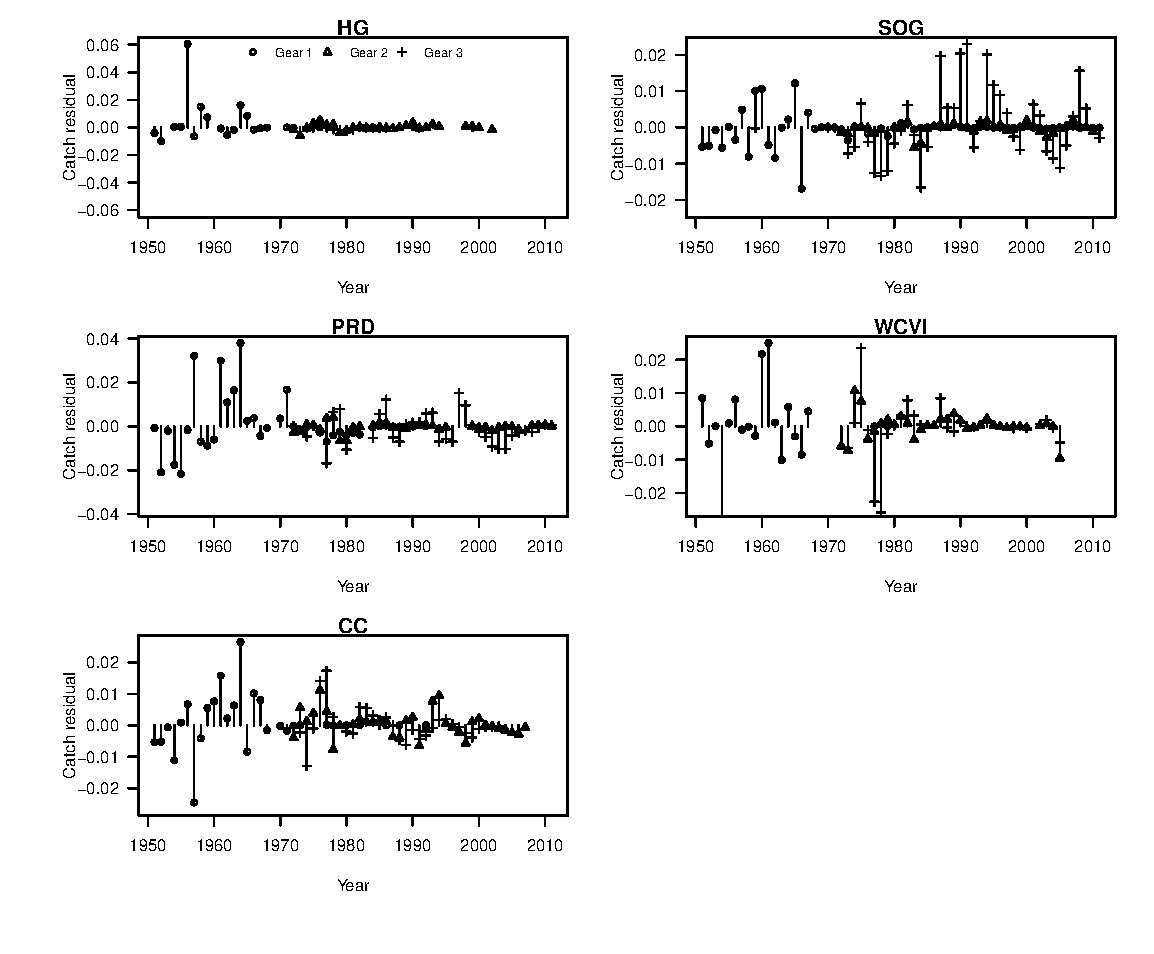
\includegraphics[width=\textwidth]{../FIGS/qPriorFigs/iscam_fig_catchresid.pdf}\\
	\caption{Residual for the log difference between observed and predicted catch for the five major SARs for each gear type (Gear 1 = winter seine fishery, Gear 2 = seine-roe fishery, Gear 3 = gill net fishery).}\label{PartII:Results:fig1}
\end{figure}


\subsubsection{Fits to the spawn survey data}
The residuals between the observed and predicted spawn survey index (on a log scale) are shown in Figure \ref{PartII:Results:fig2}.  Recall that the spawn survey data are treated as two independent time series where data between 1951--1987 were based on surface estimates of spawn area and data post 1988 are based on diver surveys of spawn area.  More weight was assigned to the contemporary data.   

For most areas, there is little pattern in the residuals between the observed and predicted survey data (Fig \ref{PartII:Results:fig2}).  For the HG, PRD and CC regions, there is very good correspondence between the observed and predicted survey data post 1988.  IN the SOG, there is a period of positive residuals between 1999 and 2005 where the predicted spawn biomass fails to increase as much as indicated by the survey.  Similary 3--4 year trends also exist in the WCVI spawn survey data after the year 2000.

\begin{figure}[!tbp]
	% Requires \usepackage{graphicx}
	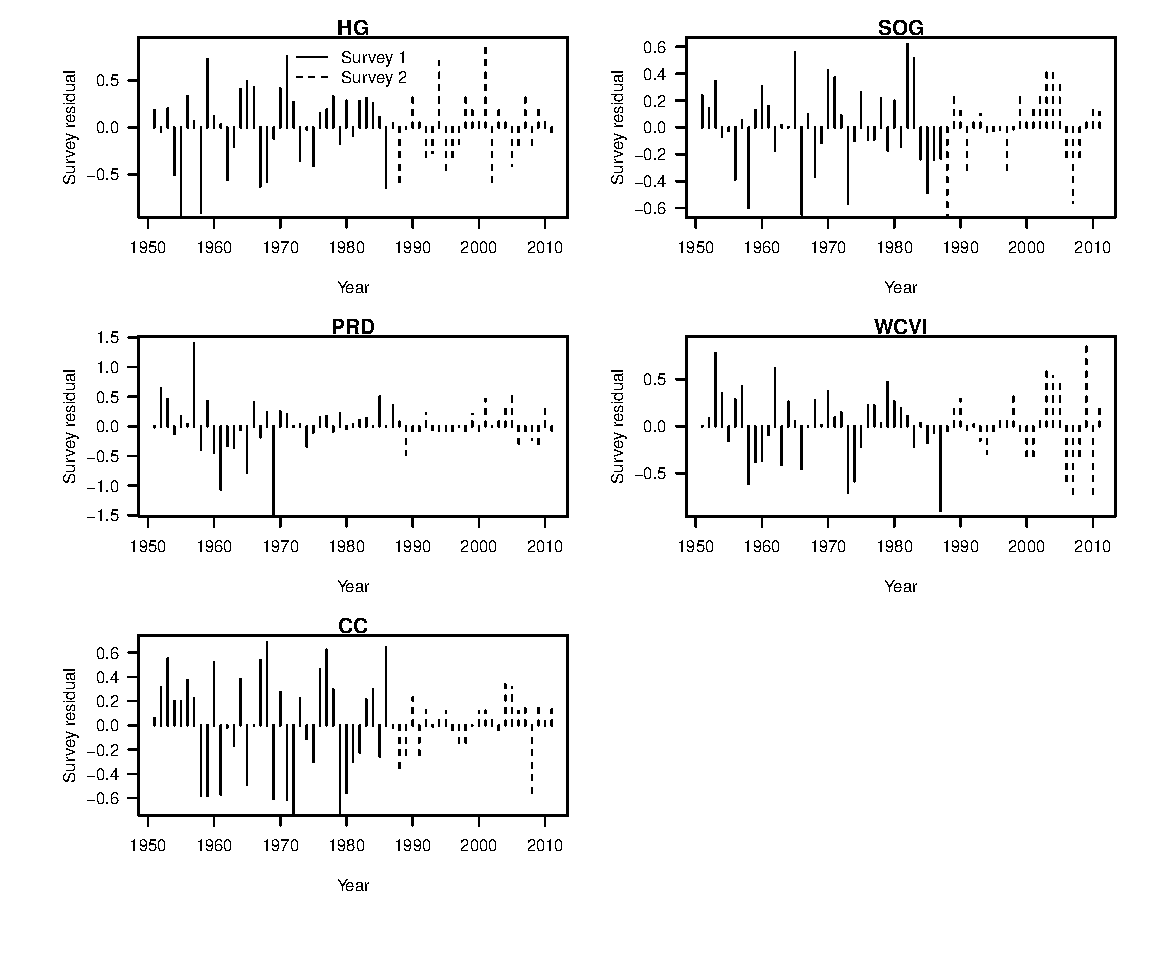
\includegraphics[width=\textwidth]{../FIGS/qPriorFigs/iscam_fig_surveyresid.pdf}\\
	\caption{Residual patterns for the log difference between observed and predicted spawn survey abundance for the five major SARs. Spawn survey data based on surface estimates are show as solid lines and data based on diver surveys is shown as dashed lines.}\label{PartII:Results:fig2}
\end{figure}

In comparison to the previous assessment for Pacific herring using the HCAM model, estimates of the catchability coefficient are very different (HCAM assumed q=1 for post 1988 data).  In each of the five major assessment regions (and the two minor regions) a less informative prior for the catchability coefficient was used (see Appendix \ref{Appendix::q_prior}).  Maximum Likelihood Estimates (MLE) of the catchability coefficients are presented for each region in Fig. \ref{PartII:Results:fig3} along with the observed and predicted trends in the spawn index.  Estimates of $q$ in both time periods are less than 1.0 for all regions with the exception of post 1988 data in the PRD region.  The interpretation of $q=1$ is that the spawn survey data is an absolute measure of spawn abundance, $q<1$ implies that the survey under-estimates the spawn abundance and $q>1$ implies an over-estimate.  For example, in the HG region the MLE values for $q$ are 0.245 and 0.433 for the pre- and post-1988 data, respectively. This could be interpreted as the spawn survey only, on average, sees 24.5\% and 43.3\% of the deposited spawn each year.  This interpretation however is conditional on the specification of mature biomass in the stock assessment model. 

\begin{figure}[!tbp]
	% Requires \usepackage{graphicx}
	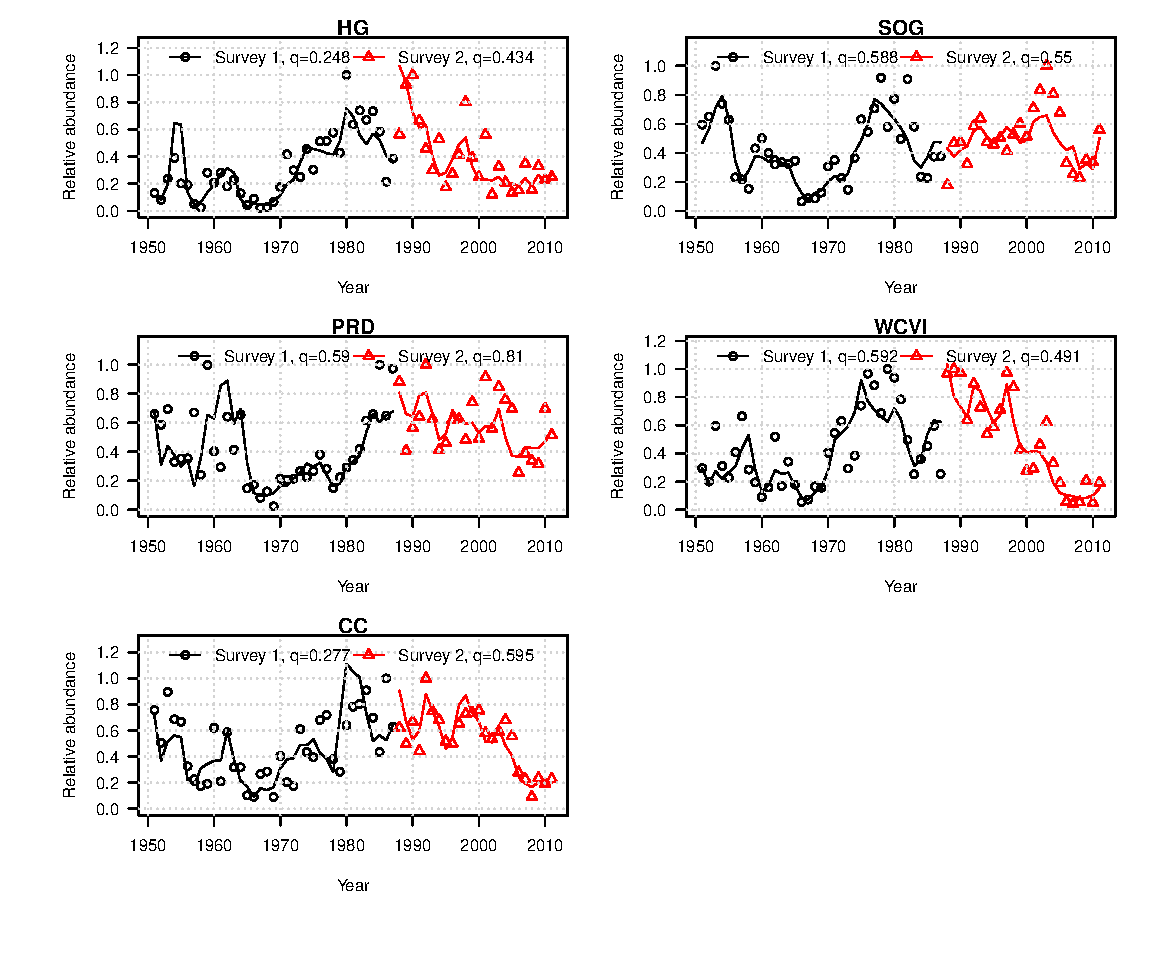
\includegraphics[width=\textwidth]{../FIGS/qPriorFigs/iscam_fig_surveyfit.pdf}\\
	\caption{Observed (points) and predicted (lines) relative abundance data (spawn survey data) for each of the five major SARs.  In each panel, the corresponding scaler ($q$) is presented for each of the surveys.}\label{PartII:Results:fig3}
\end{figure}


\subsubsection{Age composition residuals}

The assumed error distribution for the age-composition data has changed in this assessment from a multinomial distribution implemented in HCAM to a multivariate-logistic distribution. In the former implementation the age-composition data were weighted by the annual samples sizes in each region for each age and year. In the \iscam\ implementation the age-composition data for all years is given the same weight (i.e., we assume the observation errors is homogenous) based on the conditional maximum likelihood estimate of the variance (see Appendix \ref{appiSCAM} for full details).  We further pool age-proportions that are less than 2\% into the adjacent younger year class to reduce the influence of small outliers and weak cohorts.

In HG the MLE estimates of the variance for each gear is 0.102, 0.104 and 0.351, for the winter seine, seine-roe and gill net fleets, respectively (Fig. \ref{PartII:Results:figAgeCompHG}).  In general there is fairly good agreement between the observed and predicted age-composition data in this region, with poorer fits to the gill net age-composition data.  There is no persistent pattern in the residuals. 

\begin{sidewaysfigure}[!tbp]
	% Requires \usepackage{graphicx}
	\centering
	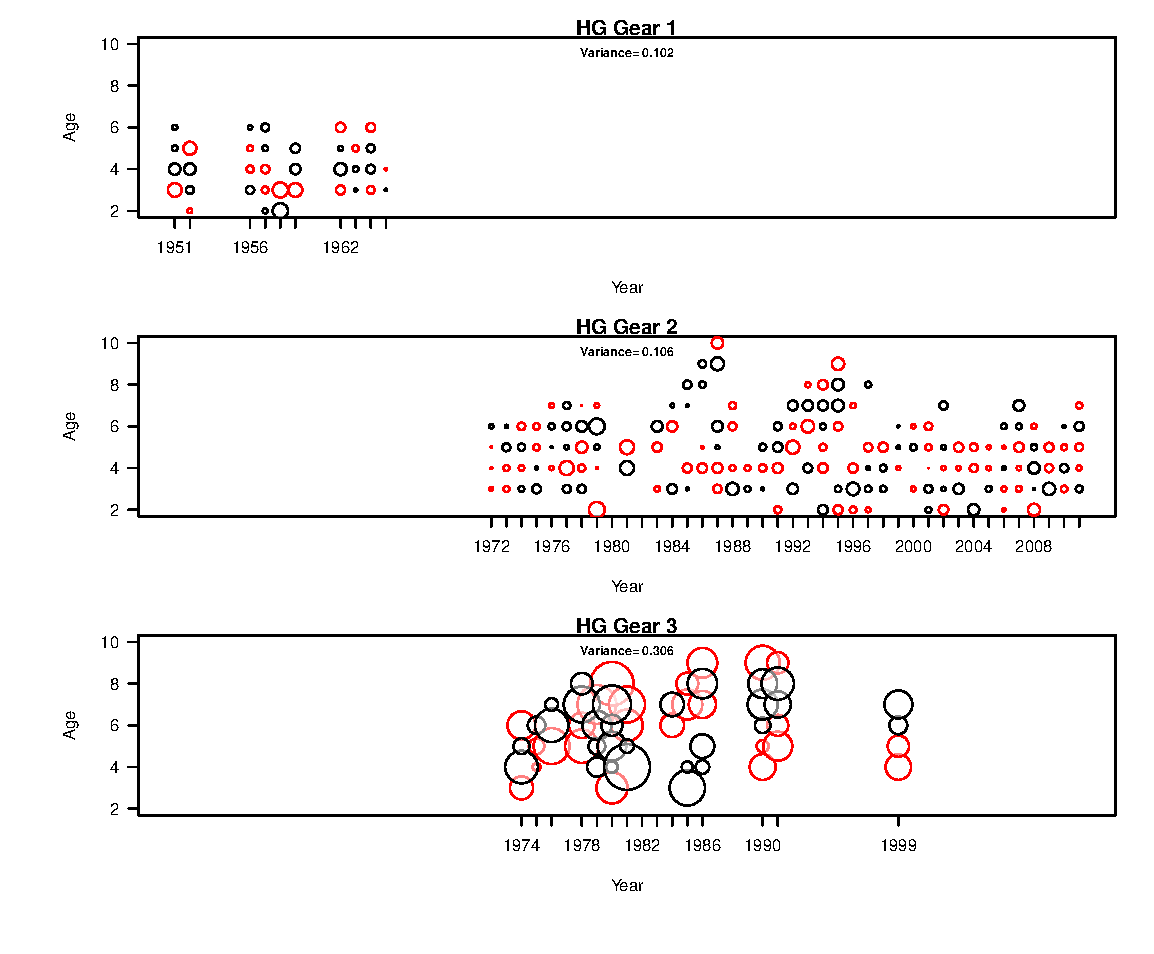
\includegraphics[width=0.9\textwidth]{../FIGS/qPriorFigs/iscam_fig_agecompsresid_HG.pdf}\\
	\caption{Residual difference between the observed and predicted proportions-at-age for HG for each of the three gear types (Gear 1 = winter seine, Gear 2 = seine-roe, Gear 3 = gill net).  The area of each circle is proportional to the residua, black is positive, and red is negative.  The corresponding MLE estimates of the residual variance is displayed in each panel.}\label{PartII:Results:figAgeCompHG}
\end{sidewaysfigure}

For the PRD region, the fits to the age-composition data are slightly poorer, with MLE estimates of the variance ranging from 0.215 to 0.358 for the seine-roe and gill net fleets (Fig. \ref{PartII:Results:figAgeCompPRD}). There is no remarkable pattern in the winter seine fishery, the seine-roe fishery tends to have positive residuals for age-3 and age 7+ fish, and negative residuals for ages 4-6 fish.  Similarly, the is an age-pattern in the residuals for the gill net fishery with negative residuals for age-4 and ages 9+ fish, and positive residuals for ages 5-8.  Residuals in 2011 age-composition data are much larger  than all other years.

\begin{sidewaysfigure}[!tbp]
	% Requires \usepackage{graphicx}
	\centering
	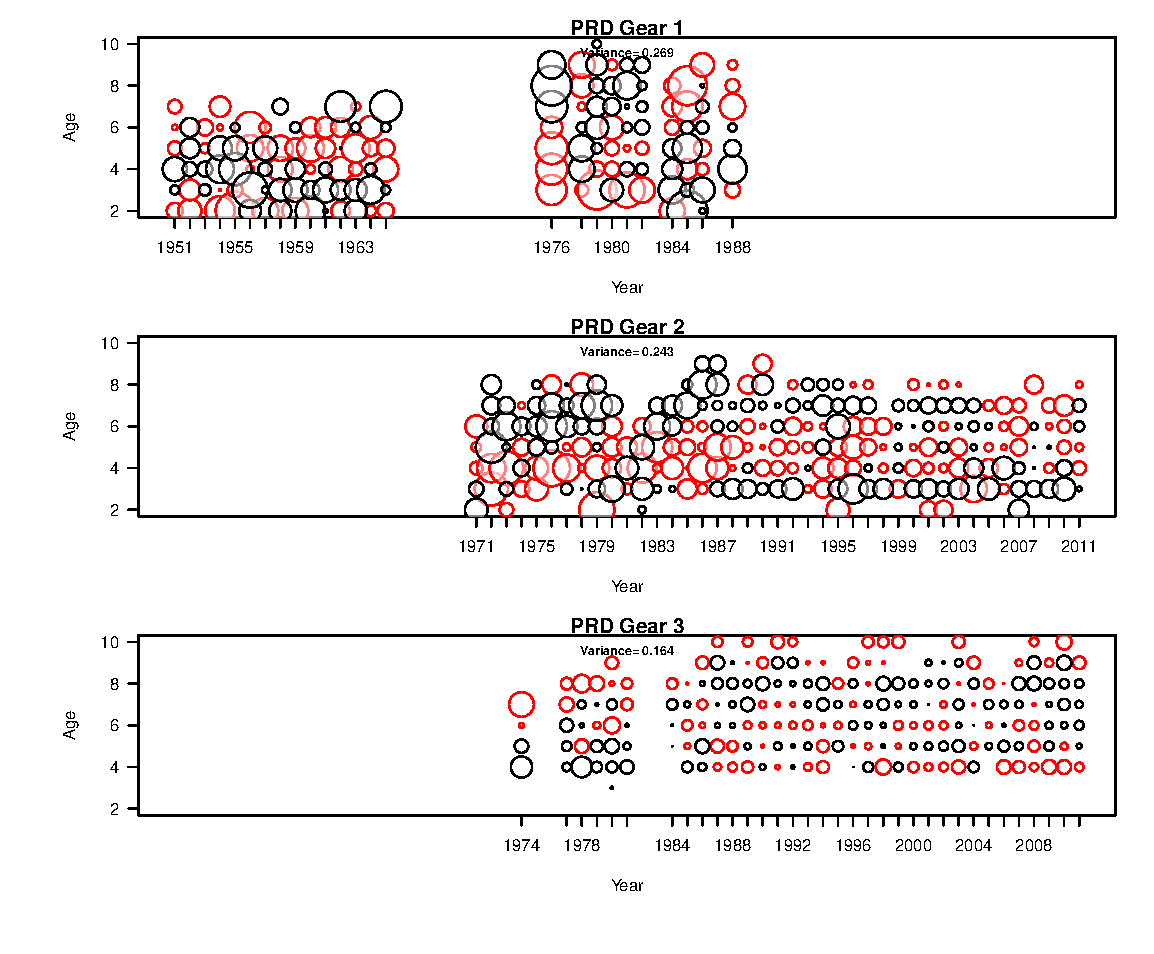
\includegraphics[width=0.9\textwidth]{../FIGS/qPriorFigs/iscam_fig_agecompsresid_PRD.pdf}\\
	\caption{Residual difference between the observed and predicted proportions-at-age for PRD for each of the three gear types (Gear 1 = winter seine, Gear 2 = seine-roe, Gear 3 = gill net).  The area of each circle is proportional to the residua, black is positive, and red is negative.  The corresponding MLE estimates of the residual variance is displayed in each panel.}\label{PartII:Results:figAgeCompPRD}
\end{sidewaysfigure}


For the Central Coast (CC) region, there is also good correspondence between the observed and predicted age-composition data, with MLE estimates of the variance ranging from 0.128 to 0.203 (Fig. \ref{PartII:Results:figAgeCompCC}).  There is no striking temporal pattern in the residuals for any of the fishing fleets.  There is a tendency to overestimate the porportion-at-age 4 and 5 in the seine-roe fishery.


\begin{sidewaysfigure}[!tbp]
	% Requires \usepackage{graphicx}
	\centering
	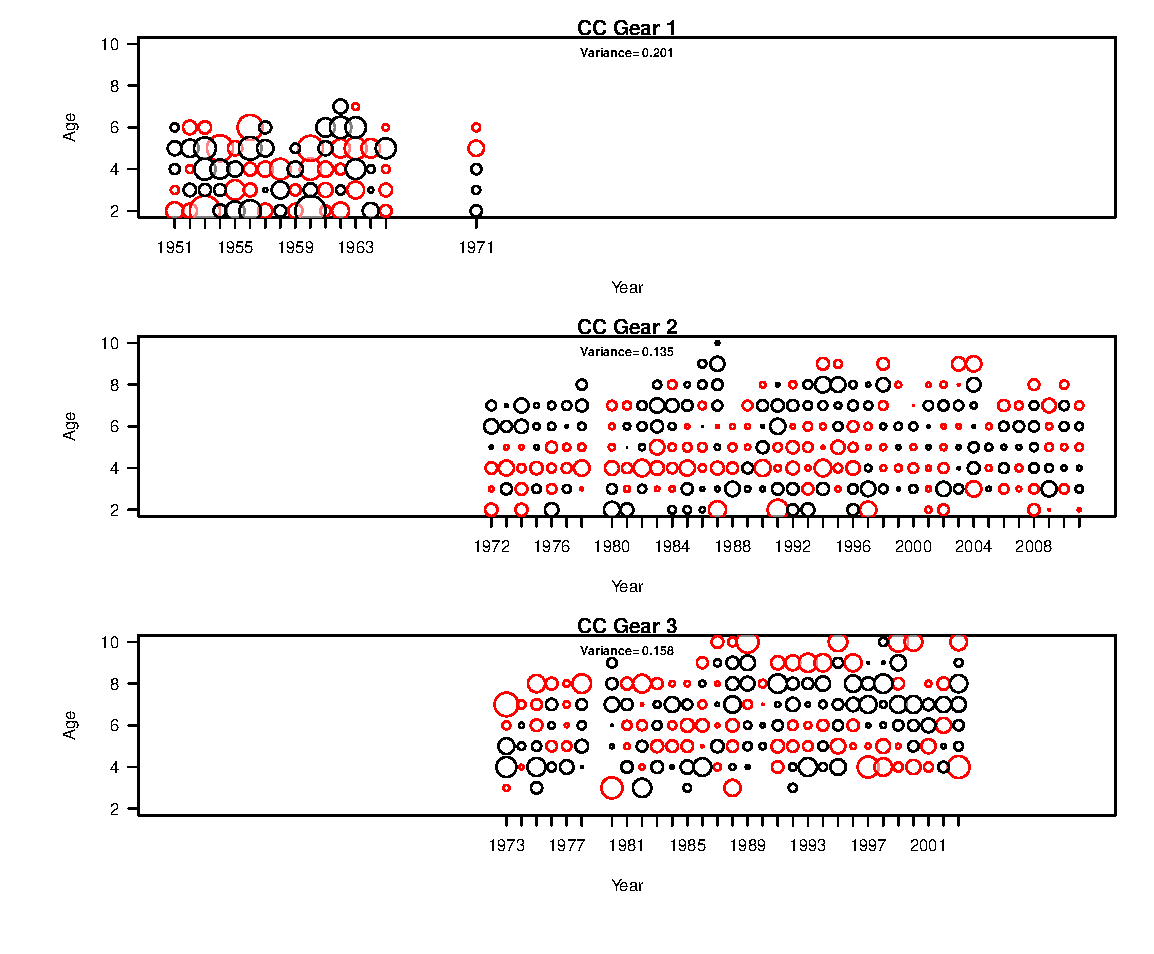
\includegraphics[width=0.9\textwidth]{../FIGS/qPriorFigs/iscam_fig_agecompsresid_CC.pdf}\\
	\caption{Residual difference between the observed and predicted proportions-at-age for CC for each of the three gear types (Gear 1 = winter seine, Gear 2 = seine-roe, Gear 3 = gill net).  The area of each circle is proportional to the residua, black is positive, and red is negative.  The corresponding MLE estimates of the residual variance is displayed in each panel.}\label{PartII:Results:figAgeCompCC}
\end{sidewaysfigure}

For the Strait of Georgia, there is also very good correspondence between the observed and predicated age-composition data for all three gears (Fig \ref{PartII:Results:figAgeCompSOG}).  The MLE estimates of the variance range from 0.088 to 0.021 for the seine-roe and gill net fleets, respectively.  In the gill net fleet  there has been a tendency to under-estimate the proportions-at-age 4-6 between the 1970s and mid 1990s and more recently to over-estimate the proportions-at-age 6-8.  Recall that selectivity for the gill net fishery is a function of the empirical weight-at-age data, which has been trending to small fish in recent years.


\begin{sidewaysfigure}[!tbp]
	% Requires \usepackage{graphicx}
	\centering
	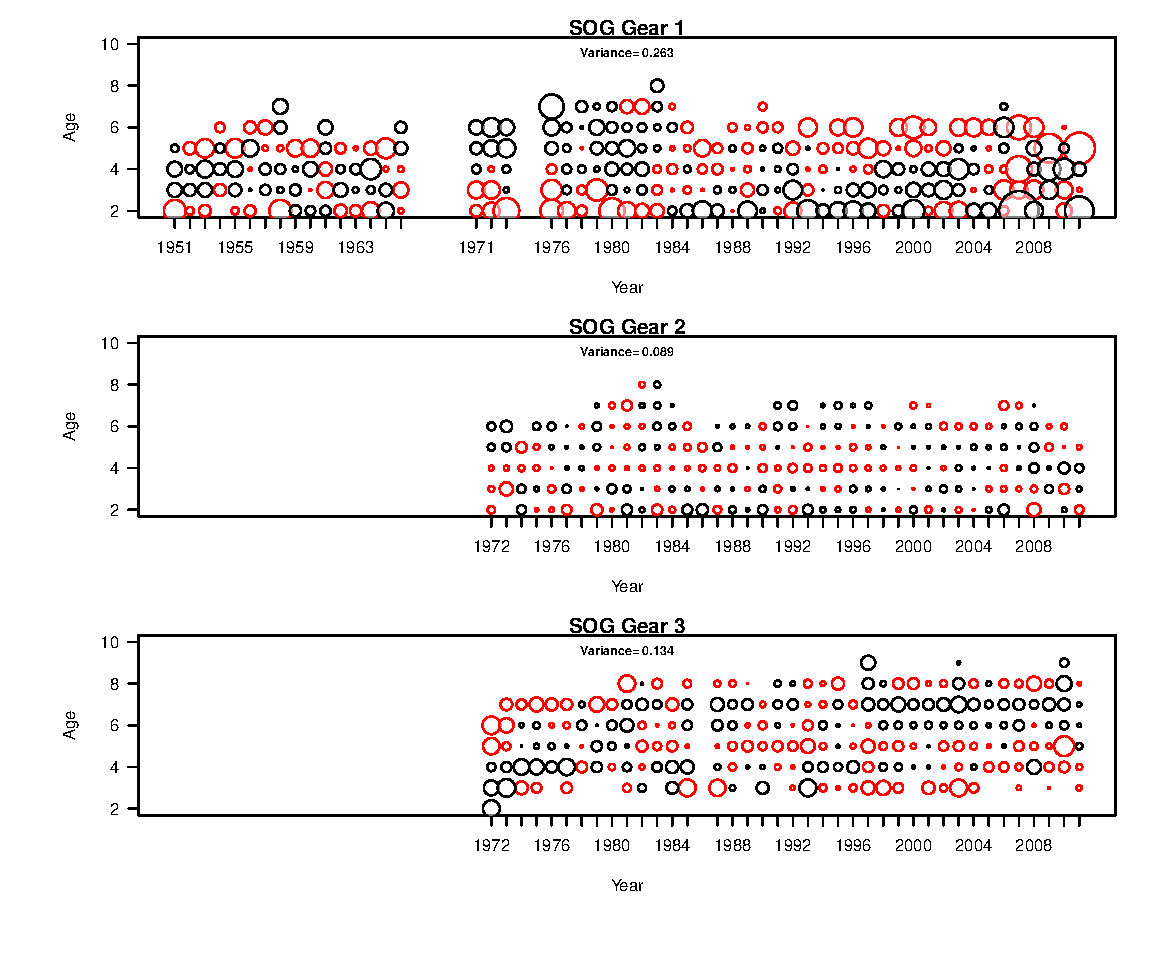
\includegraphics[width=0.9\textwidth]{../FIGS/qPriorFigs/iscam_fig_agecompsresid_SOG.pdf}\\
	\caption{Residual difference between the observed and predicted proportions-at-age for SOG for each of the three gear types (Gear 1 = winter seine, Gear 2 = seine-roe, Gear 3 = gill net).  The area of each circle is proportional to the residua, black is positive, and red is negative.  The corresponding MLE estimates of the residual variance is displayed in each panel.}\label{PartII:Results:figAgeCompSOG}
\end{sidewaysfigure}

In the case of WCVI, there is good correspondence between the observed and predicted age composition data for the seine fisheries and less so for the gill net fishery (Fig \ref{PartII:Results:figAgeCompWCVI}).  The MLE estimates of the variance range fro 0.088 to 0.314 for the seine-roe and gill net fisheries, respectively.  Residual patterns in the seine fisheries are unremarkable, perhaps an age-pattern in the seine roe fishery.  There is a tendency to under-estimate the proportions-at-age in the gill net fishery for ages 5-7.   The size of the residuals are fairly homogenous over time for all gears.


\begin{sidewaysfigure}[!tbp]
	% Requires \usepackage{graphicx}
	\centering
	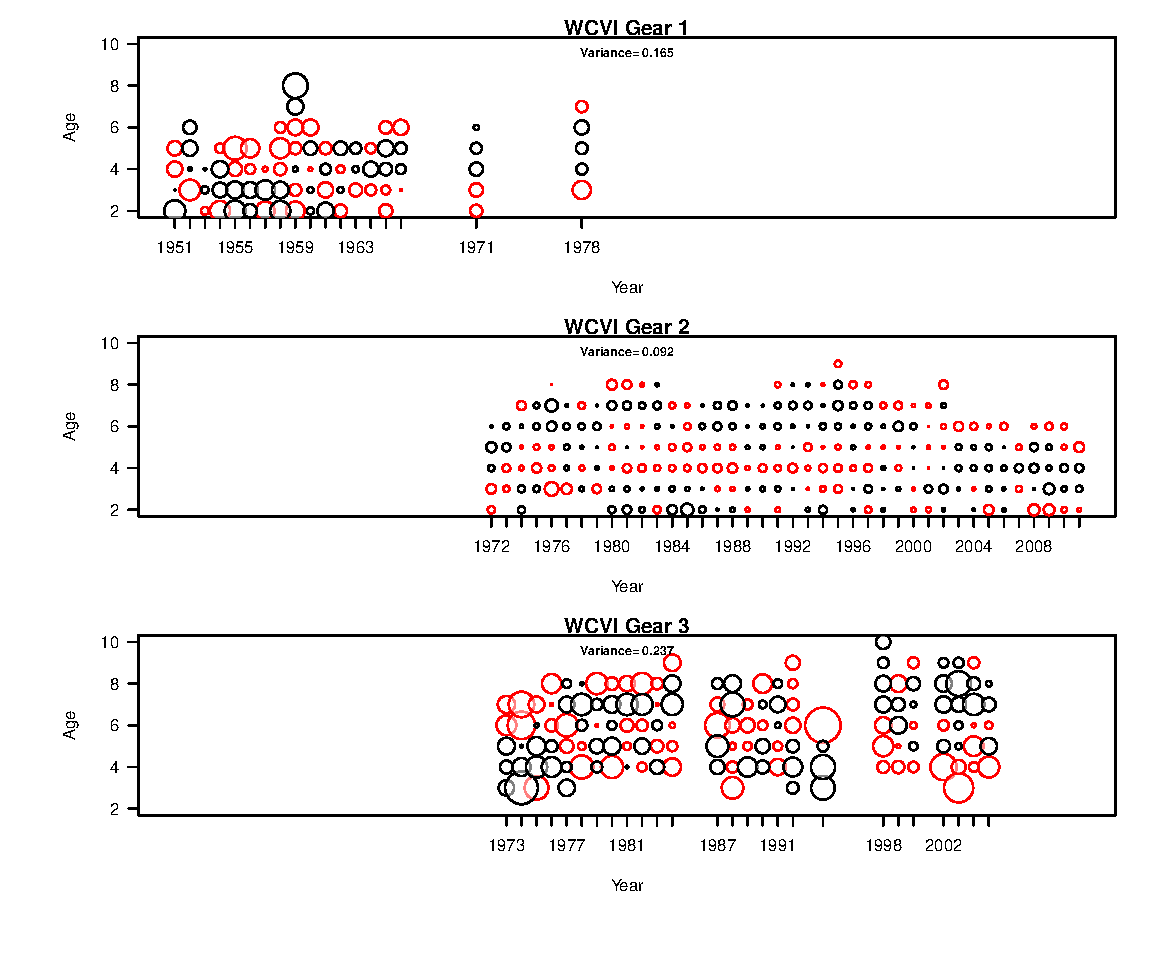
\includegraphics[width=0.9\textwidth]{../FIGS/qPriorFigs/iscam_fig_agecompsresid_WCVI.pdf}\\
	\caption{Residual difference between the observed and predicted proportions-at-age for WCVI for each of the three gear types (Gear 1 = winter seine, Gear 2 = seine-roe, Gear 3 = gill net).  The area of each circle is proportional to the residua, black is positive, and red is negative.  The corresponding MLE estimates of the residual variance is displayed in each panel.}\label{PartII:Results:figAgeCompWCVI}
\end{sidewaysfigure}







\subsubsection{Biomass estimates \& reference points}

Maximum likelihood estimates of total biomass (age 2+) and the spawning stock biomass for each of the five major assessment regions in summarized in Figure \ref{PartII:Results:figBiomass}.  Estimates of spawning stock depletion ($B_t/B_0$) for the five major regions is summarized in Figure \ref{PartII:Results:figDepletion} along with estimates of the sustainable fisheries framework reference points.  With the exception of the SOG, estimates of spawning stock depletion in 2011 are all currently below 40\% of their estimated unfished state, and in PRD, CC and the WCVI  are all estimated to be below 25\% of their unfished state (Fig \ref{PartII:Results:figDepletion}).

Spawning stock biomass in 2011 was estimated as follows: HG -- 16,789 tonnes, PRD -- 18,170 tonnes, CC -- 11,077 tonnes, SOG -- 72,135 tonnes, and WCVI -- 11,764 tonnes (Table \ref{PartII:Table1:referencePoints}).  With the exception of the PRD, these estimates are considerably higher in comparison to last years HCAM estimates; the difference largely owes to the substantial change in spawn survey scaling coefficient ($q$).

In addition to the current estimates of spawning biomass, Table \ref{PartII:Table1:referencePoints} also summarizes estimates of reference points and the total number of estimated parameters for each of the five major stock assessment regions.  Each region contained data from 1951 to 2010, and the number of estimated parameters ranges from 158 in HG to 234 in SOG.  The difference in the number of estimated parameters owes to the difference in the number of years of catch data for each region.

Estimates of unfished spawning biomass for each region is as follows: HG -- 40,960 tonnes, PRD -- 80,247 tonnes, CC -- 56,181 tonnes, SOG --- 116,023 tonnes, and WCVI -- 51,379 tonnes.  Applying the same cuttoff rule used in previous assessments (25\% of $B_0$), the results in a substantial change in the cuttoff levels for PRD, CC, SOG, and WCVI.  The previous cuttoff level for HW was estimated at 10,700 tonnes, and in this assessment there is a minor downward revision to 10,240 tonnes.  In the case of PRD, the previous cuttoff was 12,100 tonnes and in this assessment is now 20,062 tonnes.  For the CC, the previous cuttoff was 17,600 tonnes and now 14,045 tonnes.  For the SOG, the previous cuttoff was 21,200 tonnes, and in this assessment it has been revised upwards to 29,006 tonnes.  Lastly, for the WCVI the cuttoff has decreased from 18,800 tonnes to 12,845 tonnes.


% latex.default(rpTable, file = fn, title = "Stock", longtable = FALSE,      landscape = FALSE, cgroup = NULL, n.cgroup = NULL, caption = cap,      label = "TableRefPoints", na.blank = TRUE, vbar = FALSE,      size = "small") 
%
\begin{table}[!tbp]
 \small
 \caption{Summary of maximum likelihood estimates for  the 
	two minor stock areas.  No. is the total number of estimated 
	parameters, \fmsy\ the average instantaneous fishing rate to 
	achieve the maximum sustainable yield (MSY), \bo\ is the unfished 
	spawning biomass, \bmsy\ is the spawning biomass that achieves 
	maximum sustainable yield,$B_t$ is the spawning biomass at the end 
	of the 2011 fishing season, and $B_t/B_0$ is the spawning depletion 
	level at the end of the 2011 fishing season.\label{TableRefPoints}} 
 \begin{center}
 \begin{tabular}{lll}\hline\hline
\multicolumn{1}{l}{Stock}&\multicolumn{1}{c}{A2W}&\multicolumn{1}{c}{A27}\tabularnewline
\hline
No.&74&79\tabularnewline
\fmsy& 0.34&  1.9\tabularnewline
MSY&  265&  304\tabularnewline
$B_0$&2,915&2,084\tabularnewline
0.25$B_0$&  729&  521\tabularnewline
\bmsy&  705&  447\tabularnewline
0.8\bmsy&  564&  358\tabularnewline
0.4\bmsy&  282&  179\tabularnewline
$B_t$&4,671&  924\tabularnewline
$B_t/B_0$&  1.6& 0.44\tabularnewline
\hline
\end{tabular}

\end{center}

\end{table}




\begin{figure}[!tbp]
	% Requires \usepackage{graphicx}
	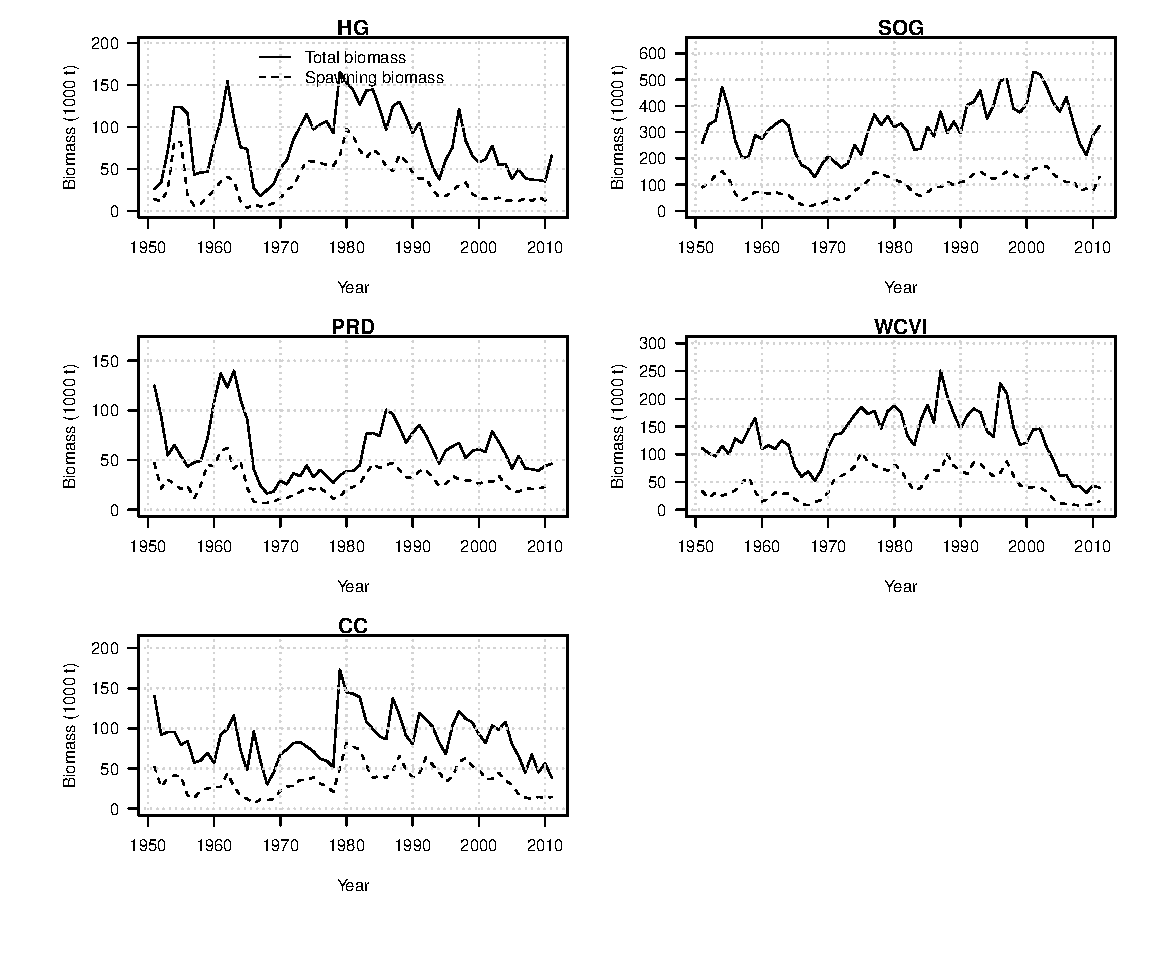
\includegraphics[width=\textwidth]{../FIGS/qPriorFigs/iscam_fig_biomass.pdf}\\
	\caption{Estimates of total biomass at the start of the year (numbers times empirical weight-at-age) and spawning stock biomass (post fishery) for the five major SARs.}\label{PartII:Results:figBiomass}
\end{figure}


\begin{figure}[!tbp]
	% Requires \usepackage{graphicx}
	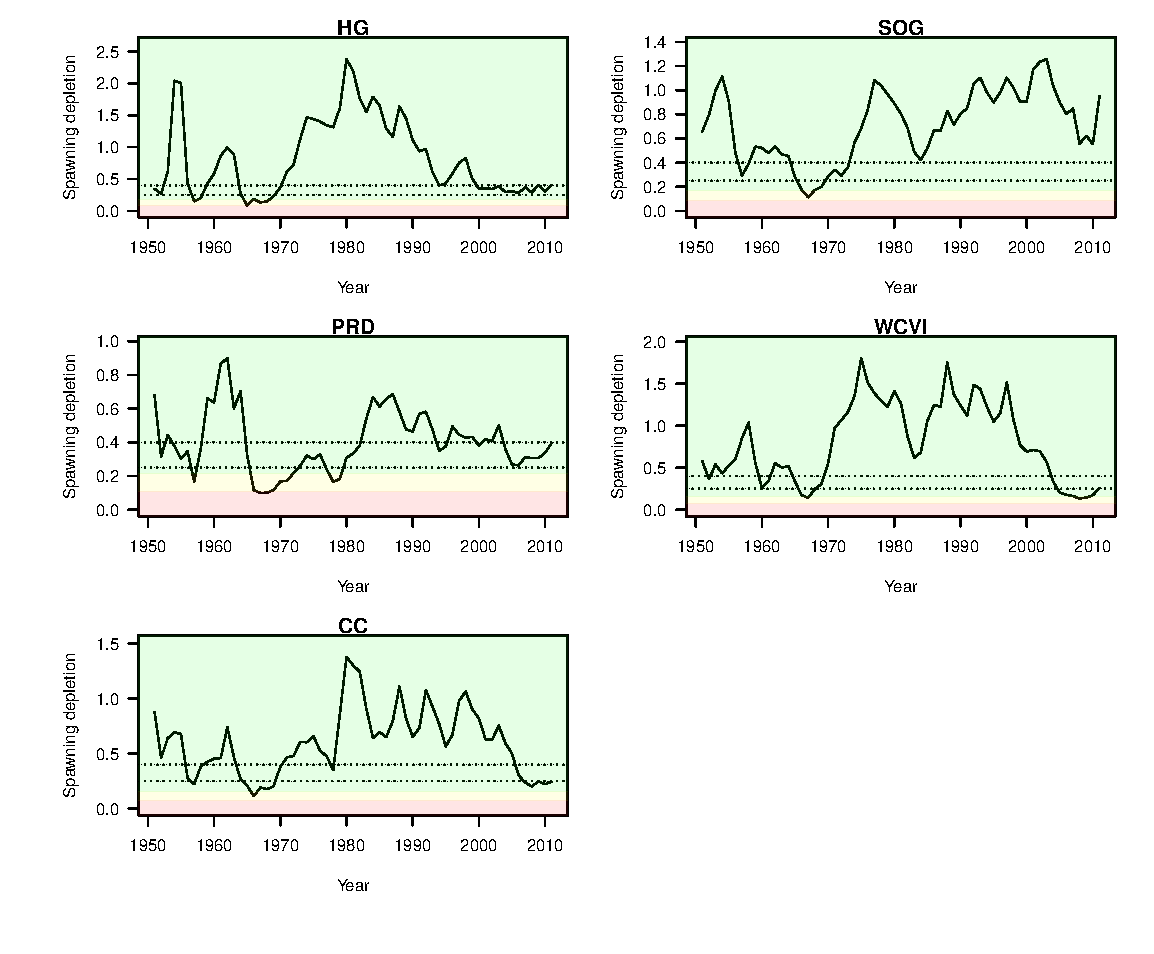
\includegraphics[width=\textwidth]{../FIGS/qPriorFigs/iscam_fig_depletion.pdf}\\
	\caption{Estimates of spawning biomass depletion ($B_t/B_0$) for each of the five major stock areas.  Horizontal dotted lines represent 25\% and 40\% depletion levels, and the shaded regions demarcate reference points based on $<$40\% \bmsy/\bo (critical zone) and 40--80\% \bmsy/\bo(cautious zone) and $>$80\% \bmsy/\bo (healthy zone).}\label{PartII:Results:figDepletion}
\end{figure}




\subsubsection{Estimates of mortality}

The most recent HCAM assessment model allowed for annual estimates of $M_t$ where natural mortality was modelled as a random walk process.  The same random walk model has been adopted in this \iscam\ implementation, however, a reduced number of parameters (12 nodes instead of 60 annual deviations) is estimated and interpolated using a bicubic spline.  The number of estimated nodes does have minor influences on the various trends in natural mortality; we came to arrive at estimating 12 nodes by ensuring the estimated trends were very similar to trends in $M$ when estimated annual natural mortality rates (NB. one could use formal model selection criterion here to determine the optimal number of nodes).

For all of the five major stock assessment regions, estimates of natural mortality rates have trended upwards since the 1950s (Figure \ref{PartII:Results:figMortality}).  Trends in estimates of natural mortality are also consistent with the trends in natural mortality from last years HCAM model  \citep[see Figure 18 in][]{Clear2010}.  In the mid to late 1970s, estimates of natural mortality rates were very low during a time when most of the stocks were recovering from the earlier reduction fishery.  In the last decade, estimates of natural mortality rates for herring have been at an all time high, and in some locations (HG, CC SOG and WCVI) there is indication that natural mortality rates may be declining. Estimates of $M_t$ in the most recent years, however,  are highly suspect because there are incomplete cohorts to infer estimates of total mortality rates.



\begin{figure}[!tbp]
	% Requires \usepackage{graphicx}
	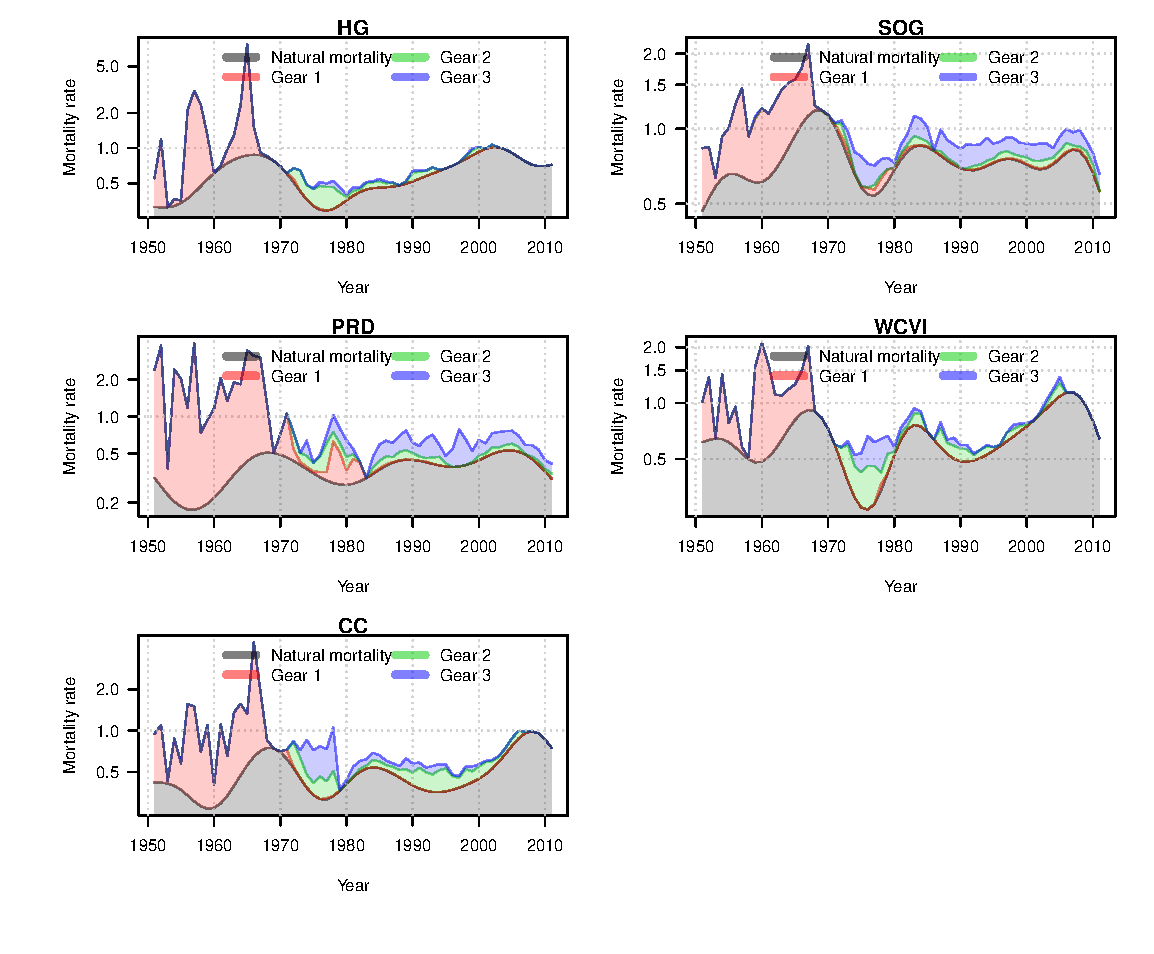
\includegraphics[width=\textwidth]{../FIGS/qPriorFigs/iscam_fig_mortality.pdf}\\
	\caption{Maximum likelihood estimates of the components of average total mortality for each of the five major stock assessment regions. Note that the y-axis is plotted on a log scale, natural mortality (grey) is age-independent, fishing mortality is age-specific and the average fishing mortality rate over all age-classes is plotted here.}\label{PartII:Results:figMortality}
\end{figure}

Estimates of fishing mortality rates in each of the regions, between 1951 and 1970 were very high due to the purse-seine fleet during the reduction fishery.  After the fishery re-opened in the early 1970s fishing mortality rates have been greatly reduced and periodic since the early 1990s due to the cuttoffs.  Of notable exception is the fishing mortality rate for the gill net fishery in PRD in the late 2000s (Fig. \ref{PartII:Results:figMortality}). This appears to be an artifact due to the structural assumption that selectivity is a function of weight-at-age.  Estimates of selectivity for the gill net fleet are all much less than 1 due to the small size of herring in the PRD region in the 2000s.

\subsubsection{Selectivity}

\subsubsection{Recruitment and stock-recruitment relationships}


\subsection{Marginal posterior distributions}

\subsection{Forecast and catch advice based on the joint posterior distribtution}
 The catch advice in Tables \ref{TableCatchAdvice} and \ref{TableCatchAdviceqFix} is based on the old cuttoffs.


% latex.default(xTable, file = fn, rowname = NULL, longtable = FALSE,      landscape = FALSE, cgroup = cgrp, n.cgroup = ncgrp, caption = cap,      label = "TableCatchAdvice", na.blank = TRUE, vbar = FALSE,      size = "small") 
%
\begin{table}[!tbp]
 \small
 \caption{Estimated spawning stock biomass,  age-4+ biomass and pre-fishery biomass for poor average and good recruitment,  cutoffs, and available harvest under the assumption that q=1 for the contemporary spawn survey data.\label{TableCatchAdviceqFix}} 
 \begin{center}
 \begin{tabular}{lllclllclclll}\hline\hline
\multicolumn{3}{c}{\bfseries }&
\multicolumn{1}{c}{\bfseries }&
\multicolumn{3}{c}{\bfseries Pre-fishery forecast biomass}&
\multicolumn{1}{c}{\bfseries }&
\multicolumn{1}{c}{\bfseries }&
\multicolumn{1}{c}{\bfseries }&
\multicolumn{3}{c}{\bfseries Available harvest}
\tabularnewline \cline{1-13}
\multicolumn{1}{c}{Stock}&\multicolumn{1}{c}{SSB}&\multicolumn{1}{c}{4+ Biomass}&\multicolumn{1}{c}{}&\multicolumn{1}{c}{Poor}&\multicolumn{1}{c}{Average}&\multicolumn{1}{c}{Good}&\multicolumn{1}{c}{}&\multicolumn{1}{c}{Cutoff}&\multicolumn{1}{c}{}&\multicolumn{1}{c}{Poor}&\multicolumn{1}{c}{Average}&\multicolumn{1}{c}{Good}\tabularnewline
\hline
HG& 7,147& 2,736&& 4,259& 6,662&12,776&&10,700&&     0&     0& 2,076\tabularnewline
PRD&29,071& 8,427&&10,486&12,649&20,016&&12,100&&     0&   549& 4,003\tabularnewline
CC& 8,427& 4,308&& 6,720& 9,264&15,438&&17,600&&     0&     0&     0\tabularnewline
SOG&51,500&21,640&&31,921&40,236&52,616&&21,200&& 6,384& 8,047&10,523\tabularnewline
WCVI& 6,948& 3,645&& 7,404&11,373&18,438&&18,800&&     0&     0&     0\tabularnewline
\hline
\end{tabular}

\end{center}

\end{table}



% latex.default(xTable, file = fn, rowname = NULL, longtable = FALSE,      landscape = FALSE, cgroup = cgrp, n.cgroup = ncgrp, caption = cap,      label = "TableCatchAdvice", na.blank = TRUE, vbar = FALSE,      size = "small") 
%
\begin{table}[!tbp]
 \small
 \caption{Estimated spawning stock biomass,  age-4+ biomass and pre-fishery biomass for poor average and good recruitment,  cutoffs, and available harvest based on a normal prior ($\mu=0,\sigma=0.274$) for $q$ in both surveys.\label{TableCatchAdvice}} 
 \begin{center}
 \begin{tabular}{lllclllclclll}\hline\hline
\multicolumn{3}{c}{\bfseries }&
\multicolumn{1}{c}{\bfseries }&
\multicolumn{3}{c}{\bfseries Pre-fishery forecast biomass}&
\multicolumn{1}{c}{\bfseries }&
\multicolumn{1}{c}{\bfseries }&
\multicolumn{1}{c}{\bfseries }&
\multicolumn{3}{c}{\bfseries Available harvest}
\tabularnewline \cline{1-13}
\multicolumn{1}{c}{Stock}&\multicolumn{1}{c}{SSB}&\multicolumn{1}{c}{4+ Biomass}&\multicolumn{1}{c}{}&\multicolumn{1}{c}{Poor}&\multicolumn{1}{c}{Average}&\multicolumn{1}{c}{Good}&\multicolumn{1}{c}{}&\multicolumn{1}{c}{Cutoff}&\multicolumn{1}{c}{}&\multicolumn{1}{c}{Poor}&\multicolumn{1}{c}{Average}&\multicolumn{1}{c}{Good}\tabularnewline
\hline
HG&10,474& 7,147&& 9,241&12,159&19,292&&10,700&&     0& 1,459& 3,858\tabularnewline
PRD&17,754&11,125&&13,092&15,210&21,643&&12,100&&   992& 3,042& 4,329\tabularnewline
CC& 6,441& 2,486&& 4,366& 6,487&11,538&&17,600&&     0&     0&     0\tabularnewline
SOG&50,927&26,807&&38,502&49,288&65,667&&21,200&& 7,700& 9,858&13,133\tabularnewline
WCVI& 3,835& 1,284&& 4,447& 7,688&13,333&&18,800&&     0&     0&     0\tabularnewline
\hline
\end{tabular}

\end{center}

\end{table}



% latex.default(xTable, file = fn, rowname = NULL, longtable = FALSE,      landscape = FALSE, cgroup = cgrp, n.cgroup = ncgrp, caption = cap,      label = "TableCatchAdvice", na.blank = TRUE, vbar = FALSE,      size = "small") 
%
\begin{table}[!tbp]
 \small
 \caption{Estimated spawning stock biomass,  age-4+ biomass and pre-fishery
			biomass for poor average and good recruitment,  cutoffs,  and 
			available harvest based on median values from the joint posterior distribution for the two minor areas.  All units are reported in tonnes.\label{TableCatchAdvice}} 
 \begin{center}
 \begin{tabular}{lllclllclclll}\hline\hline
\multicolumn{3}{c}{\bfseries }&
\multicolumn{1}{c}{\bfseries }&
\multicolumn{3}{c}{\bfseries Pre-fishery forecast biomass}&
\multicolumn{1}{c}{\bfseries }&
\multicolumn{1}{c}{\bfseries }&
\multicolumn{1}{c}{\bfseries }&
\multicolumn{3}{c}{\bfseries Available harvest}
\tabularnewline \cline{1-13}
\multicolumn{1}{c}{Stock}&\multicolumn{1}{c}{SSB}&\multicolumn{1}{c}{4+ Biomass}&\multicolumn{1}{c}{}&\multicolumn{1}{c}{Poor}&\multicolumn{1}{c}{Average}&\multicolumn{1}{c}{Good}&\multicolumn{1}{c}{}&\multicolumn{1}{c}{Cutoff}&\multicolumn{1}{c}{}&\multicolumn{1}{c}{Poor}&\multicolumn{1}{c}{Average}&\multicolumn{1}{c}{Good}\tabularnewline
\hline
HG&15,202&10,080&&12,917&16,623&26,056&&     0&& 1,292& 1,662& 2,606\tabularnewline
PRD&14,859&10,272&&12,132&14,262&20,908&&     0&& 1,213& 1,426& 2,091\tabularnewline
CC& 7,213& 2,631&& 4,801& 7,044&12,470&&     0&&   480&   704& 1,247\tabularnewline
SOG&58,691&30,882&&47,169&59,423&76,324&&     0&& 4,717& 5,942& 7,632\tabularnewline
WCVI& 5,187& 1,691&& 5,745& 9,593&16,057&&     0&&   575&   959& 1,606\tabularnewline
\hline
\end{tabular}

\end{center}

\end{table}





%Decision table
Notes from June Meeting:\\
Were not completely comfortable with the q estimates, but we believe the approach used to develop the informative prior for q is better than the ad hoc q=1 assumption.  Assuming $q=1$ is more conservative as there is a tendency for $q<1$ when freely estimated with an informative prior.


% Statisitcal fit

% Retrospective performance.

% Estimated reference points.

\section*{Results} % (fold)
\label{sec:results}

\subsection*{Statisical fit} % (fold)
\label{sub:statisical_fit}

Statisitics summarizing how well each model fits a single realization of simulated data are based on the overall objective function value, Deviance Information Criterion (DIC) and the Root Mean Square Error (RMSE) between observed and predicted quantities (Table \ref{tab:statisticalPeformance}). Under conditions in which the true selectivity is fixed (scenmario 1), similar fits to the relative survey abundance index and age-composition data (see Survey RMSE and Survey age RMSE in Table \ref{tab:statisticalPeformance}) were obtained  irrespective of the form of the assumed selectivity curve for the commercial fishery.  However, fits to the commercial age-composition data markedly improved under the time-varying age-based selectivity model (c).  Allowing for additional structure in the selectivity coefficients over time resulted in decreases in the RMSE from 0.47, 0.40 and 0.32 for models (a), (b), and (c), respectively for the commercial age-composition information (Table \ref{tab:statisticalPeformance}).  The worst fit to the commercial age-composition was obtained for the bicubic spline model (d).

We do not recommend basing model selection solely on statistical criterion, such as DIC, but for statistical comparison we provide DIC and $\Delta$DIC values to give a sense of the relative differences between the various assessment models for each simulation case.  In the cases examined here (Table \ref{tab:statisticalPeformance}), DIC always favors the most structurally complex model (c) with the largest number of estimated selectivity parameters. The large improvement in fit for model (c) is always due to explaining more residual variation in the age-composition data. All other models appear to fit the survey index and age-composition equally, regardless if the data were generated from fixed selectivities or complex time-varying selectivities.  This is not an unexpected result, as the observation models for the survey age composition data are structurally consistent with the simulation model.  What is significant is that the use of the conditional maximum likelihood estimate of the variance to weight the commercial age-composition data is down-weighted when the incorrect selectivity model is specified for the commercial selectivities. Even though our examples show a small effect moving from fixed selectivity to block-selectivites (RMSE increases from 0.47 to 0.52, Table \ref{tab:statisticalPeformance}), increasing the number of selectivity blocks could exacerbate this effect. Note also, that this down-weighting incorrectly assigns process error to observation error due to mis-specification of selectivity.




\begin{table*}[!tbh]
	\caption{Statistical performance based on the objective function value, effective number of estimated parameters, DIC, $\Delta$DIC, Root Mean Square Error (RMSE) in recruitment deviations, survey abundance residuals, and the age-composition residuals for models fit to fixed, discrete time blocks and continous changes in commercial selectivity.}
	\label{tab:statisticalPeformance}
	\begin{center}
		\begin{tabular}{l|cccc}
		\hline

		\hline
		\textbf{} & \textbf{Fixed (a)} & \textbf{Discrete (b)} & \textbf{Continuous (c)} & \textbf{Bicubic spline (d)} \\
		\hline

		
	    \multicolumn{5}{l}{\textbf{\underline{True selectivity is fixed}}}\\
		Objective function            &  -836.41 &  -918.16 & -1208.16 &  -939.17 \\
		Eff. No. parameters             &    96 &   116 &   334 &   173 \\
		DIC              & -1479.77 & -1601.51 & -1739.09 & -1528.01 \\
		$\Delta$DIC         &   259.32 &   137.58 &     0.00 &   211.08 \\
		Recruitment RMSE &     1.04 &     1.04 &     1.06 &     1.04 \\
		Survey RMSE      &     0.25 &     0.25 &     0.26 &     0.26 \\
		Commercial RMSE         &     0.47 &     0.40 &     0.32 &     0.49 \\
		Survey age RMSE         &     0.24 &     0.25 &     0.25 &     0.24 \\
		%Total.RMSE       &     2.03 &     1.96 &     1.90 &     2.06 \\
		
		\hline
		\multicolumn{5}{l}{\textbf{\underline{True selectivity has 3 time blocks}}}\\
		Objective function            &  -775.49 & -1051.57 & -1335.82 & -1028.80 \\
		Eff. No. parameters             &    96 &   116 &   337 &   173 \\
		DIC              & -1356.24 & -1868.57 & -1990.44 & -1707.88 \\
		$\Delta$DIC         &   634.20 &   121.87 &     0.00 &   282.56 \\
		Recruitment RMSE &     1.04 &     1.04 &     1.05 &     1.05 \\
		Survey RMSE      &     0.26 &     0.26 &     0.26 &     0.26 \\
		Commercial RMSE         &     0.52 &     0.35 &     0.29 &     0.45 \\
		Survey age RMSE         &     0.25 &     0.29 &     0.25 &     0.24 \\
		%Total.RMSE       &     2.10 &     1.92 &     1.86 &     2.02 \\

		\hline
		\multicolumn{5}{l}{\textbf{\underline{True selectivity changes annually}}}\\
		Objective function            &  -717.56 &  -788.52 & -1029.41 &  -785.91 \\
		Eff. No. parameters             &    96 &   116 &   333 &   173 \\
		DIC              & -1241.22 & -1342.26 & -1382.43 & -1222.14 \\
		$\Delta$DIC         &   141.21 &    40.17 &     0.00 &   160.29 \\
		Recruitment RMSE &     1.06 &     1.09 &     1.12 &     1.05 \\
		Survey RMSE      &     0.26 &     0.26 &     0.27 &     0.26 \\
		Commercial RMSE         &     0.52 &     0.44 &     0.35 &     0.56 \\
		Survey age RMSE         &     0.27 &     0.29 &     0.30 &     0.27 \\
		%Total.RMSE       &     2.14 &     2.10 &     2.07 &     2.17 \\



		% Objective function  & -1452.78 &  -1461.06 &  -1695.12 &  -1538.09 \\
		% Eff. No. parameters &    96    &    110    &    344    &    175    \\
		% DIC                 & -2712.84 &  -2701.20 &  -2696.89 &  -2723.12 \\
		% $\Delta$DIC         &    10.28  &    21.92 &     26.23 &      0.00 \\
		% Recruitment RMSE    &     1.03 &      1.03 &      1.03 &      1.03 \\
		% Survey RMSE         &     0.25 &      0.26 &      0.25 &      0.25 \\
		% Commercial RMSE     &     0.28 &      0.28 &      0.20 &      0.26 \\
		% Survey age RMSE     &     0.26 &      0.26 &      0.27 &      0.26 \\

		
		% \hline
		% Objective function  & -1340.49 &  -1428.81 &  -1689.57 &  -1516.78 \\
		% Eff. No. parameters &    96    &    109    &    345    &    175    \\
		% DIC                 & -2487.96 &  -2638.03 &  -2683.48 &  -2680.78 \\
		% $\Delta$DIC         &   195.52 &     45.45 &      0.00 &      2.70 \\
		% Recruitment RMSE    &     1.04 &      1.04 &      1.03 &      1.03 \\
		% Survey RMSE         &     0.25 &      0.26 &      0.25 &      0.25 \\
		% Commercial RMSE     &     0.32 &      0.29 &      0.20 &      0.26 \\
		% Survey age RMSE     &     0.26 &      0.26 &      0.27 &      0.26 \\

		
		% \hline
		% Objective function  & -1293.30 &  -1304.14 &  -1543.59 &  -1376.39 \\
		% Eff. No. parameters &    95    &    109    &    344    &    177    \\
		% DIC                 & -2394.61 &  -2387.88 &  -2393.28 &  -2396.33 \\
		% $\Delta$DIC         &     1.72 &      8.45 &      3.05 &      0.00 \\
		% Recruitment RMSE    &     1.13 &      1.13 &      1.12 &      1.12 \\
		% Survey RMSE         &     0.26 &      0.27 &      0.27 &      0.27 \\
		% Commercial RMSE     &     0.30 &      0.30 &      0.21 &      0.28 \\
		% Survey age RMSE     &     0.33 &      0.34 &      0.33 &      0.32 \\

		\hline

		\hline
		\end{tabular}
	\end{center}
\end{table*}
The effective number of estimated parameters is based on the difference between the expectation of the deviance and the deviance based on the expectation of the parameter values.  The larger the effective number of parameters is a measure of how well the model fits the data.  In all cases the effective number of parameters was equal to or greater than the number of parameters estimated in the model.  In the case of model (c) the effective number of parameters ($\approx$335) is much greater than the 319 that were actually estimated in the ADMB code.  However, it should also be noted that the variance parameters for age-composition residuals and the scaling parameter $q$ \citep[see][]{walters1994calculation} are based on the conditional maximum likelihood estimates, rather than explicitly estimating them inside the model code.  This parameterization implies an additional 67 parameters and hence the effective number of parameters is much less than the 386 parameters in model (c).  Again, we caution the use of DIC for model selection in cases where data are weighted via conditional maximum likelihood estimate of the variance.


% For the cases where the true selectivity is based on a fixed logistic function, the most appropriate model based on DIC is model (d) where a bicubic spline is used to model selectivity. The RMSE terms for model (d) are less than the true underlying values that were used to generate the data, which is of no surprice when additional flexibility in selectivity can accomodate some of the residual variance in age-composition in the form of minor changes in selectivity (Table \ref{tab:statisticalPeformance}).   This pattern of explaining the residual variation is virtually the same regardless of what the true underlying selectivity pattern is.

% In the case where the true selectivity changes discretely over three time blocks, assessment models with time-varying selectivity (c) and (d) appear to fit the data better that models that assumed fixed selectivity (a), or even the discrete changes in selectivity (see $\Delta$DIC values in Table \ref{tab:statisticalPeformance}).  For this particular case, it's better to allow for continous changes in selectivity than to 
% assume fixed values.

% In the case where the true selectivity changes annually, based on relative cohort abundance, the model results were a bit more surprising.  The expectation would be that assuming fixed selectivity would perform less well than allowing for time-varying selectivity.  Based on the $\Delta$DIC values obtained in Table \ref{tab:statisticalPeformance} there is very little differnce between models that allow for continous changes in selectivity (models c and d) and fixed selectivity (model a).  There was less weight for the model that allows for discrete-block changes in selectivity (model b).

% Similar results were also obtained in the case where true selectivity changes annually (as a function of the relative cohort abundance).  However, the difference between assuming block selectivity and fixed selectivity resulted in negligble differences in the $\Delta$AIC values.  Moreover, the RMSE for the age-composition data was greater than the true values used to generate the observation errors in age-sampling in models (a) and (b). For model (c), the RMSE was less than the true value for the commercial age-composition, and  in model (d) it was identical to the true value.   

% subsection statisical_fit (end)
\subsection*{Retrospective performance} % (fold)
\label{sub:retrospective_performance}

Two useful graphical tools for examining retrospective problems in stock assessment models are referred to here as spaghetti plots (Fig. \ref{fig:retrospectiveSSB}), and squid plots (Fig. \ref{fig:retrosquidbase}), respectively.  In the spaghetti plots, successive estimates of spawning stock biomass based on sequentially removing the terminal year of data for four previous years are overlayed on each panel.  In addition to the estimated spawning biomass in Fig. \ref{fig:retrospectiveSSB}, the true spawning biomass that was used to generate simulated data is also shown for reference.  In the squid plots, successive estimates of spawning biomass relative to the  spawning biomass in the terminal year of data are overlaid.  In Fig. \ref{fig:retrosquidbase}, the percent bias is shown as the relative difference between the true values; hence a 100\% bias implies that the stock size is over-estimated by a factor of 2.  


\begin{figure*}[!tbh]
	\begin{center}
		\includegraphics[angle=0,width=\textwidth]{FIGRetroSpectiveSSB.eps}
	\end{center}
	\caption{One realization of retrospective estimates of spawning biomass for simulated Pacific hake populations where four years of data was sequentially removed from.  The true spawning biomass used to simulated the data is included for reference.}
	\label{fig:retrospectiveSSB}
\end{figure*}

Based on the maximum likelihood results from a single realization shown in Fig. \ref{fig:retrospectiveSSB}, there is a tendency for the model to systematically over-estimate the spawning stock biomass in the terminal years.  This trend is largely a function of the recent downward trend in abundance since the mid 2000s, and is also related to mis-specification of the selectivity curve.  Self-consistent simulation and assessment  models tend to have lest retrospective bias than the misspecified models (Figure \ref{fig:retrospectiveSSB}).  In the case of the true selectivity being fixed over time, the least amount of retrospective bias occurred in the simple models (a) and (b), and the largest bias was observed for model (c).  Similar results were also obtained in the discrete changes in selectivity (row 2 of Fig. \ref{fig:retrosquidbase}) as well as the time-varying changes in selectivity.  Also of interest is the retrospective behavior in model (d) where the sequential removal of the terminal year data results in changing the knot positions in the bicubic spline (see early years on column (d) of Fig. \ref{fig:retrosquidbase}). Retrospective  estimates of spawning biomass earlier in the time series of model (d) are slightly more variable in comparison to models with fixed selectivities (a), (b), and even in the case where selectivity is allowed to vary annually (c).  However, these results are from a single realization, and should not be used to make general inferences in retrospective bias.  Median values from a series of Monte Carlo trials would be more appropriate for making general inferences.  These results from a single realization merely illustrate that despite additional structural flexibility associated with time-varying selectivity, large retrospective bias can still occur. 



% For the simulated data based on fixed selectivity, the qualitative pattern in retrospective bias was similar for all four alternative selectivity scenarios (Figure \ref{fig:retrospectiveSSB}, 1a, ..., 1d).   The worst performing models were the cases with continuous changes in selectivity over time (1c and 1d), with maximum estimates of retrospective bias relative to the terminal values approaching 25\% for the bicubic spline model (Figure \ref{fig:retrosquidbase}).  

% For cases based on simulated data with discrete time blocks in selectivity, the least amount of bias was observed in the case where the correct model was specified (Figure \ref{fig:retrosquidbase}, 2b).  Assuming fixed selectivity or continuous changes in selectivity resulted in significantly more retrospecitve bias.  Assuming fixed selectivity also resulted in further departures from the true spawning biomass in the initial years.

\begin{figure*}[!tbh]
	\begin{center}
		\includegraphics[angle=0,width=\textwidth]{FIGRetroSquidBase.eps}
	\end{center}
	\caption{One realization of retrospective estimates of bias in spawning biomass relative to spawning biomass estimated with all available data.  These biases are based on the same spawning biomass trajectories in Figure \ref{fig:retrospectiveSSB}.}
	\label{fig:retrosquidbase}
\end{figure*}


% \begin{figure}[tb]
% 	\begin{center}
% 		\includegraphics[angle=90,width=0.85\textwidth]{.fig:RetroSquid.png}
% 	\end{center}
% 	\caption{Retrospective estimates of bias in spawning biomass relative to the true spawning biomass used to simulated the data.  These biases are based on the same spawning biomass trajectories in Figure \ref{fig:retrospectiveSSB}.}
% 	\label{fig:retrosquid}
% \end{figure}

% In the cases where the true selectivity varies over time, the retrospective performance was least biased for the models that assume time-varying selectivity (Figure \ref{fig:retrosquidbase}, 3c and 3d).  Retrospective peformance is much worse if the selectivity is assumed to be constant, or change in a series of blocks, when the real underlying process is continuous change in selectivity (Figure \ref{fig:retrosquid}, 3a and 3b). 

% Monte Carlo retrospective results. Make general statement that less retrospective bias when assuming more structural complexity.  May be better to assume a penalized random walk in selectivity than to not.

Over a number of Monte Carlo trials (40 independent data sets) the patterns in retrospective bias over the alternative selectivity assumptions differ from the single realization shown in Fig. \ref{fig:retrospectiveSSB}.  To quantify retrospective bias, a series of summary statistics were used to measure the trade-off between precision and bias in the retrospective analyses (Table \ref{tab:RetroStatistics}).  The mean bias $\mu$ reflects the average difference between the terminal and retrospective year spawning biomass and is generally lowest for models that allow for time-varying selectivity (models (c) and (d) in Table \ref{tab:RetroStatistics}).  The absolute mean bias $|\mu|$ better characterizes the mean retrospective  variation.  For example, in model 3c (Table \ref{tab:RetroStatistics}) the mean bias $\mu$ is relatively small, but the mean absolute difference over four retrospective years is very large.  This is also reflected in the summary statistic $\Omega$ and the Mean Absolute Deviation (MAD).  Even though model 3c is the correct model for the simulations with continuous changes in selectivity, the results in Table \ref{tab:RetroStatistics} suggest that model 3d would be preferable due to less mean bias and a lower overall variance in the potential bias.  

\begin{table*}[!tbh]
	\caption{Retrospective bias statistics for each model run, where $\mu_1$ corresponds to the mean bias over four retrospective years, $\mu_2$ is the absolute mean, $\Omega$ is a combined measure of mean and absolute bias, and MAD is the Mean Absolute Deviation of $\mu_2$.  Lower MAD scores imply less variability in retrospective bias estimates.}
	\label{tab:RetroStatistics}
	\begin{center}
	\begin{footnotesize}
		
		\begin{tabular}{l|cccc|cccc|cccc}
		\hline

		\hline
		&\multicolumn{4}{c|}{\textbf{Fixed}} & \multicolumn{4}{c|}{\textbf{Discrete}} & \multicolumn{4}{c}{\textbf{Continous}} \\
		&\textbf{1a}  &\textbf{1b}  &\textbf{1c}  &\textbf{1d}  &\textbf{2a}   &\textbf{2b}  &\textbf{2c}  &\textbf{2d}  &\textbf{3a}  &\textbf{3b}  &\textbf{3c}  &\textbf{3d}\\
		\hline
		$\mu_1$     &-9.14& -8.26& -1.55& -1.77& -8.88& -12.57& -1.11& -3.11& -6.72& -5.90& -2.09& -0.83\\
		$\mu_2$ &14.19& 13.63& 13.46& 12.78& 12.94&  14.96& 12.12& 13.75& 14.06& 14.08& 17.99& 13.85\\
		$\Omega$  &19.13& 18.28& 17.49& 16.53& 17.58&  20.66& 15.73& 17.86& 18.62& 18.47& 22.97& 18.08\\
		MAD    & 4.77&  4.68&  6.42&  4.93&  5.32&   6.28&  5.11&  5.48&  4.73&  4.84& 10.51&  5.78\\

		\hline

		\hline
		\end{tabular}
	\end{footnotesize}
	\end{center}
\end{table*}

Similar results were also obtained for the simulations involving fixed selectivities and discrete time blocks with less overall mean bias, and lower MAD's, for models with continuous changes in selectivity over time (Table \ref{tab:RetroStatistics}).


% subsection retrospective_performance (end)


\subsection*{Estimated reference points} % (fold)
\label{sub:estimated_reference_points}


The impacts of model specification on the estimates of MSY-based reference points are summarized using a series of box-plots (Fig. \ref{fig:RefPointBias}) based on Monte Carlo trials.  In each box plot the $\ln$ ratios of the estimated versus true values are shown where the median bias is based on the solid bar.  In the case where the true model is based on fixed selectivity, estimated reference points are relatively unbiased ($\pm$ 10\%); however, the precision of the estimates decreases with increasing model complexity (Fig. \ref{fig:RefPointBias}).  There is a bit of a trend in the estimate of $F_{\rm{MSY}}$ that corresponds to an increase in overall stock productivity with assumed increases in model complexity.  This same increasing trend is also present, but less pronounced, in the estimates of MSY.  These trends indicate that the overall scale and productivity of the estimated population increases with increasing model complexity. 

In cases where the true model is based on scenario 2, estimated $F_{\rm{MSY}}$ reference points were biased upwards for model (a)  because the true selectivity shifts towards smaller fish later in the time series (Fig. \ref{fig:RefPointBias}). The vast majority of the age-composition data were based on selectivities curves that target larger fish and the constant selectivity assumption in model (a) does not capture this trend. Estimates of MSY were less biased in this case. Estimates of spawning biomass reference points ($B_{\rm{MSY}}$ and $B_o$) were less sensitive to the assumed model structure, with the exception of model (a) being fit to scenario 2. Recall that the MSY-based reference points are based on selectivity values in the terminal year. Under the assumption of constant selectivity, estimates of $F_{\rm{MSY}}$ are almost certain to be biased with the rare exception that the terminal year selectivity corresponds to the estimated average selectivity.  

\begin{figure*}[!tbh]
	\begin{center}
		\includegraphics[width=\textwidth]{FIGRefPointBias.eps}
	\end{center}
	\caption{Estimates of precision and bias for fishing mortality rate reference points ($F_{\rm{MSY}}$), maximum sustainable yield (MSY), spawning biomass as MSY ($B_{\rm{MSY}}$) and the unfished spawning biomass ($B_o$) based on Monte Carlo trials using data simulated from fixed, discrete blocks and continuous changes in selectivity. }
	\label{fig:RefPointBias}
\end{figure*}

For the case where the true model involves continuous changes in selectivity, or scenario 3, estimates of $F_{\rm{MSY}}$ for all models are biased upwards (Fig. \ref{fig:RefPointBias}).  Estimates of $F_{\rm{MSY}}$ are more variable for models that have a large number of estimated selectivity parameters, indicating that estimates of selectivity in the terminal year are highly imprecise (recall that MSY-based reference points were based on estimated selectivity in the terminal year). All other reference points are much less biased if a more complex assessment model is assumed in comparison to the underlying simulation model.


% RMSE resultz
In all of the Monte Carlo simulation-estimation experiments the variance components for recruitment deviations, survey index errors, age-composition data for both the commercial and survey samples were estimated.  The root mean square error (RMSE) of the residuals is a proximate measure of how each of the data series are weighted internally in the assessment model.   The distribution of the RMSE values for each error component is shown in Fig. \ref{fig:RMSEdist} for scenarios 1-3 using models (a)-(d).  The RMSE values for the survey abundance index for all scenario and model combinations were very similar to the true standard deviation of 0.3 that was used to generate the simulated observation errors (Fig. \ref{fig:RMSEdist}).   For scenarios (1) and (2), the RMSE value for the recruitment deviations were also similar to the true standard deviation of $\sigma_R=1.12$ in the simulated recruitment deviations.  For scenario (3) however, RMSE values were greater than 1.12 under the assumption that selectivity changes annually  as in model (c), but less so under model (d) where changes selectivity is constrained via the bicubic spline interpolation.

\begin{figure*}[!tbh]
	\begin{center}
		\includegraphics[width=\textwidth]{FIGRMSEdist.eps}
	\end{center}
	\caption{Distribution of Root Mean Squared Error values for the recruitment deviations, survey residuals, commercial and survey age-composition residuals based on 40 Monte Carlo trials.}
	\label{fig:RMSEdist}
\end{figure*}

The pattern of RMSE values for the commercial age composition samples generally decreases with increasing flexibility in the selectivity model (Fig. \ref{fig:RMSEdist}, lower left panel), with the exception of the bicubic spline model.  The simulated size-based selectivities in all of the model scenarios was very dynamic owing to the large changes in the empirical size-at-age data in Pacific hake (Fig. \ref{fig:simSelex}). The bicubic spline model used in model (d) estimates a total of 60 knots (7 for age, and 12 for years), and interpolates over age, not size-at-age.  In this case, the bicubic spline performs rather poorly in comparison to fixed size-based selectivities and the annual age-based selectivity due to the tension imposed by the limited number of knots.

Another pattern in the distributions of RMSE values shown in Fig. \ref{fig:RMSEdist} that is of significant interest is how the weight of the survey age-composition data changes with changes in assessment models.  In scenario 1 and 2, the distribution of RMSE values is fairly similar for all assessment models, and here we note that the variability in RMSE values increases with increasing number of estimated selectivity coefficients.  However, in scenario (3) with continuous changes in commercial selectivity being the true case, the relative RMSE values increase (i.e., poorer fit) for the survey age-composition data.  In other words, more structurally complex assessment models fit the commercial age-composition better at the partial expense of putting less weight on the survey age-composition.  But note that the RMSE values for 3c are roughly equal to the true standard deviation of $\sigma_2=0.3$ in the multivariate logistic sampling distribution.  

For model (d), relatively poor fits were obtained for the commercial age-composition data, and RMSE values for this model were much larger than model (c).  However, model (d) fit the survey age-composition data better and does not allow for increased process errors in the form of recruitment deviations in comparison to model (c).  In short, annual changes in selectivity greatly improves the fit to commercial age-composition data, but this comes at the expense of poorer fits to the survey age-composition data and increased recruitment variation. Note also, that the performance of these time-varying selectivity models also depends on correctly specifying the appropriate penalty weights to constrain the amount of smoothing that occurs.  Cross-validation studys such as that of \cite{maunder2011using} could be a useful approach in the process of determining the appropriate weighting schemes.


% The distribution of the RMSE values from the Monte Carlo trials displayed pretty consistent patters over each alternative dataset (Figure \ref{fig:RMSEdist}).  The residual fit to the survey abundance index was very similar across all simulated datasets and all alternative assessment models.  The true coefficient of variation used in simulating the true data was fixed at 0.3, and accounting for the bias correction in the lognormal errors, the theoretical RMSE in the residuals should be approximately 0.255.  The standard deviation in the simulated recruitment residuals was fixed at 1.12 and the distribution of RMSE values is very similar for the fixed selectivity and time-block selectivity simulated datasets (Figure \ref{fig:RMSEdist}).  In the case where the simulated data was based on continouse changes in selectivity, the RMSE values for the recruitment deviations was slightly higher than the true value, presumably to allow for more variation in recruitment that could be explained by annual changes in selectivity.

% The pattern of RMSE values for the commercial age-composition residuals was consistent across simulated datasets, where largest RMSE values were always observed with fixed selectivity (Figure \ref{fig:RMSEdist}, model a), and the smallest under the annual time-varying selectivity (Figure \ref{fig:RMSEdist}, model c).  Models with intermediate complexity were able to explain more residual variation in the comercial age-composition(models b and d, respectively).  

% subsection estimated_reference_points (end)

\subsection*{Simulation performance} % (fold)
\label{sub:simulation_performance}




To qualitatively evaluate how each of the four alternative selectivity models would perform if the analyst was na\"ive about the underlying true selectivity, we use a simple rank order system (Table \ref{tab:rankorder}).  For example, if DIC was the statistical basis for choosing the most appropriate selectivity model then based on the simulation results in Table \ref{tab:statisticalPeformance} when the true underlying model is based on fixed selectivity, the rank order of DIC values (low to high) is model c, b, d, and a. If the underlying model is not known, the DIC criterion favors model (c) the most, and model (d) the second most.    Based on all of the criterion listed in Table \ref{tab:rankorder}, the most appropriate model to choose if in fact the analyst was na\"ive about the underlying processes in selectivity would be model (c).    Model (b) also ranks fairly high; however, this assumes the correct block time-periods can be identified from residual analysis or historical knowledge of fishing practices.

\begin{table*}[!tbh]
	\caption{Ranking of model based on Deviance Information Criterion, RMSE, retrospective bias and bias in the estimates of $F_{\rm{MSY}}$ and MSY based on Monte Carlo trials. Each column ranks the assumed selectivity model from most likely (left) to least likely (right) for simulation case study.  The top-two ranks represent the most and second most frequently selected model.}
	\label{tab:rankorder}
	\begin{center}
		\begin{tabular}{l|ccc|c}
		\hline

		\hline
		\textbf{Criterion} & \textbf{Fixed} & \textbf{Discrete} &\textbf{Continuous} & \textbf{Top-two ranks} \\
		\hline
		DIC from Tab. \ref{tab:statisticalPeformance}
		           & c,b,d,a & c,b,d,a & c,b,d,a & c,b\\
		\hline
		Retrospective    & d,c,a,b & c,d,a,b & d,a,b,c & c,d\\
		$F_{\rm{MSY}}$   & b,c,a,d & c,d,b,a & c,b,a,d & c,b\\
		MSY              & d,c,b,a & c,d,b,a & d,a,c,b & d,c\\
		RMSE             & c,b,a,d & c,b,a,d & c,b,a,d & c,b\\
		% RMSE           & c,d,a,b & c,d,b,a & c,d,a,b & c,d\\
		% Retrospective  & d,b,a,c & d,a,c,b & a,b,d,c & d,b\\
		% $F_{\rm{MSY}}$ & c,d,a,b & c,d,a,b & a,b,d,c & c,d\\
		\hline

		\hline
		\end{tabular}
	\end{center}
\end{table*}

% subsection simulation_performance (end)

% section results (end)





	% %!TEX root = /Users/stevenmartell/Documents/iSCAM-project/fba/Halibut/WRITEUP/Halibut.tex

\section{Discussion} % (fold)
\label{sec:discussion}

The overarching objective of this study was to investigate the impacts of bycatch reduction in the BSAI and Gulf of Alaska on the halibut yields, exploitable biomass, spawing biomass and wastage in the directed commercial fishery.  This was accomplished by using a sex/age-structured simulation model to account for future biomass and fishing mortality rates under alternative hypotheses about future recruitment and growth rates of halibut.  The simulation model was, in part, parameterized using estimates of numbers-at-age and sex in the 1996, age-1 recruits from 1996--2006, empirical length-at-age data from the setline survey, a length-weight relationship from a recent study and fishing mortality rates from the directed fishery, 032, U32, recreational and personal use fishing fleets.  All of these parameter inputs were taken from the most recent IPHC assessment of Pacific halibut \citep[see][wobblesq model]{Hare2012Rara}.  The simulation model did not perfectly replicate estimates of exploitable biomass in the IPHC assessment largely due to the differences in the average weight-at-age data.  


The IPHC assessment model uses empirical weight-at-age data obtained from the commercial fishery catch.  At ages 6-10 the mean weight-at-age data samples are largely biased towards faster growing (larger) fish that are of legal size.  For the purposes of simulating future biomass, it was not possible to come up with a simple procedure to replicate this size-selective process.  In lieu, growth curves for female and male halibut were constructed from the empirical length-at-age data obtained in the setline survey between 1996--2011.  Simulated weight-at-age data was then based on the allometric length-weight relationship developed by \cite{courcellesre}.  The net result of using this growth curve is that simulated exploitable biomass between 1996-2011 was scaled downwards.  The overall trends between the biomass simulated in this study and the IPHC assessment were nearly identical.  This difference in projected biomass would change the overall scale of the simulated results, but would have very little influence on the relative changes in simulated exploitable biomass (and spawning biomass) over the two alternative management procedures that involve reducing the bycatch of non-targeted fisheries in the BSAI, or the Gulf of Alaska.


There are alternative approaches to modelling density-dependent growth.  In the case adopted in this model, growth rates of individual cohorts are established at birth and are strictly a function of the density of that cohort relative to the average cohort density.  The reason for adopting this approach, rather than a time-varying approach, is that it conveniently does not allow for individual fish to shrink in length.  Unfortunately, this assumption does not allow for growth rates of individual cohorts to change in response to changing environmental conditions (if they were also modelled) or changes in the density of cohorts associated with fishing.  For example, it may be plausible that growth rates of an individual cohort may increase over time as the density of halibut is reduced through natural and fishing mortality rates.  Growth rate responses to changes in density have been observed in many experimental populations of rainbow trout in freshwater lakes \citep{post1999density}. 

The results of the bycatch reductions in the BSAI and GOA regions do not appear to have much of an influence on the coastwide estimates of exploitable biomass and spawning biomass.  The principle reason is that for every pound of reduced bycatch, there is a corresponding increase in the directed fishery.  However, it appears that the directed fishery has more of an impact on the exploitable biomass than the bycatch fishery.  This was demonstrated by the ratio of lost yield in the directed fishery per pound of bycatch taken by other fisheries.  Or in other words, 10 pounds of bycatch removed is roughly equivalent to 9 pounds of yield lost to the commercial fishery. 

Another important point about bycatch impacts on the halibut stocks lies in the small regional scale.  In both this simulation model and the assessment model developed by the IPHC, there is no explicit  or implicit spatial representation of the large-scale management areas.  Unfortunately, it is not possible to examine how reducing bycath in area 4CDE, would affect the exploitable biomass, spawning biomass, wastage, etc.  in the specific areas.  Migration and movement of halibut between the management areas, and the lack of information about migration,  is one of the primary reasons why the coastwide assessment model was adopted.  It is possible that a reduction in bycatch in a specific area, may provide a local increase in exploitable biomass and impact catch rates in the directed fishery.  But at this time data are insufficient to capture these small scale dynamics.

In summary, reducing halibut bycatch by 50\% in the BSAI or GOA regions by 2.7 million pounds has no large impacts on the projected estimates of coastwide spawning biomass or exploitable biomass.  Further, this reduction of 2.7 million pounds results in about a 2.5 million pound increase in the directed fishery; simulated yield loss ratios were less than 1.0 and are a function of the current age-structure in the population.  The directed commercial fishery is by far the largest component of total mortality in the coastwide assessment model; information is lacking to determine the impacts of various fisheries at smaller spatial scales.

% section discussion (end)


	\section*{Discussion} % (fold)
\label{sec:discussion}

% Summary of the study
The over-arching objective of this simulation study was to compare the performance of assuming more structural complexity in selectivity when in fact the real data come from a simple stationary process, and assuming simple structural complexity when real data come from a fishery with dynamic changes in selectivity.  To address this objective, a simulation model conditioned on length-based selectivity and variable length-at-age by year was used to generate simulated data for four alternative assessment models that assumed: (a) selectivity was length-based and stationary, (b) selectivity was length-based and changed discretely in four time periods, and (c) selectivity was age-based and allowed to change each year, and (d) selectivity was age-based and interpolated over age and year using a bicubic spline and 60 equally spaced knots.  From the perspective of a na\"ive analyst who is unfamiliar with the history of the fishery and the source of the catch-age data, adopting a penalized time-varying selectivity may be more appropriate than assuming constant selectivity.  This general result is also consistent with a similar simulation study that examined time-varying changes in catchability \citep{wilberg2006performance}.

The addition of age-composition information into stock assessments greatly enhances the estimability of the underlying production function and related reference points \citep{magnusson2007mfd}.  In addition, age-composition information can also contribute to the estimation of over-all population scale via catch-curves and fixed assumptions about natural mortality and fisheries selectivity.  However, as assumptions about natural mortality and selectivity are relaxed (and freely estimated), information about population scaling degrades \citep{hilborn1992quantitative}. If the relative abundance index available for fitting lacks contrasting information to resolve confounding between overall productivity and population scale, the move towards more flexible selectivity models will lead to greater uncertainty.  In such cases where it is known that selectivity has changed over time, the addition of prior information on population scaling (i.e., priors for $B_o$ or survey $q$) will particularly valuable. 

Earlier versions of the multivariate logistic likelihood for the age-composition data added a small fixed constant (1.e-30) to the observed and predicted age-proportions to ensure that the function remained defined when observed proportions-at-age were equal to 0 (i.e., this was done to avoid taking the natural logarithm of 0).  It turns out that the value of the fixed constant would have slight influences on the results and in some cases prevent the non-linear search routine from converging to a solution.  Adding a small constant to 0-observations that are likely to have high measurement error is akin to imputing data and is probably not a safe practice in the long-run.  As an alternative approach, we adopted a method used by \cite{richards1997visualizing} where observed 0 proportions-at-age (or some minimum proportion, e.g., 2\% in their paper) were pooled with the adjacent year class for that year only.  For example, if the observed proportion of age-4 fish in 1985 was equal to 0, the estimation model would compute the likelihood for the number of age 4--5 fish in 1986;  there is no likelihood component for age-4 fish in 1985.  This pooling of year classes eliminates the need for adding small, potentially influential, constants to the likelihood. There is also a small caveat on this pooling approach: if a given cohort never appears in catch-age data (i.e., a complete year-class recruitment failure), the estimation model will equally split the year class into the adjacent cohort.  Thus in choosing an appropriate threshold, we recommend that this number be sufficiently small so as not to allow adjacent cohorts to be pooled over their life-span.  Also, the users should conduct sensitivity analyses to this threshold value to ensure the results are robust.

Changes in selectivity over time are also a special case of time-varying catchability.  It has already been demonstrated that additional sources of information, such as tagging data \citep{martell2002implementing}, and/or area swept information \citep{winters1985interaction}, would reduce the confounding between stock size and stock productivity.  Statistical catch-at-age models rely on a separability assumption where year and age effects in the observed catch-at-age data can be partitioned into fishing mortality and selectivity, respectively.  Having auxiliary information on either one of these effects from area-swept estimates of relative fishing mortality or size-based selectivity based on tag return data would reduce potential confounding and improve the estimability of time-varying parameters \citep[e.g.,][]{sinclair2002disentangling}.

This simulation study examined the specific case where the true underlying selectivity is length-based and the corresponding age-based selectivity changes over time due to changes in growth rates.  Selectivity is a product of vulnerability and availability.  Vulnerability is the probability of catching a fish at a given time/location assuming the fish is available to harvest.  Availability is the probability of fish being present in the time/location where fishing activity is occurring.  These two processes are completely confounded and cannot be separated without additional information that directly measures either vulnerability or availability.  As a result of these two processes, the definition of fisheries selectivity may have many subtle differences among fisheries, or even among years in a given fishery.  Moreover, changes in harvest policy, or changes in allocation among regulatory areas, or fishing fleets, can result in dramatic changes in age-based selectivity due to time/area interactions between various fishing fleets and stock distribution.  Given such complexities, it might be preferable to always adopt an age-based time-varying selectivity sub model in statistical catch-age assessments. Initial assessments could start with very high penalty weights to constrain how much selectivity is allowed to vary (e.g., $\lambda^{(3)}$), then begin to relax the penalty and examine the sensitivity of both model fit and policy performance to the assumed penalty weight.  Simply assuming a fixed selectivity model, or even block selectivities, is akin to extremely large penalty weights on time-varying selectivity.  In this regard, this simulation presented a 'worst-case' scenario for time-varying selectivity.  Future work could simulate the application of time-varying selectivity in conjunction with a set of rules governing adjustment of the $\lambda^{(3)}$  and directly explore its performance (i.e., Table \ref{tab:rankorder}).

One potential concern with the addition of more and more selectivity coefficients is that the assessment model begins to over-fit the age-composition data and explain the observed data with additional recruitment variation and more complex selectivity coefficients. More complex datasets including estimates of CVs for indices or effective sample sizes for composition information could limit overfitting and ensure the root mean squared errors are consistent with the measured or assumed values.  This overfitting result was observed in the Monte Carlo simulations in this study where the underlying data were generated with extremely complex selectivity patterns and the estimation model had a very flexible selectivity model with many estimated parameters.  Such an over-parameterized model would be of less utility in forecasting due to large uncertainties and confounding in selectivity and recruitment deviations in the terminal year. However, the true uncertainty would be better represented, which might lead to more realistic expectations in a decision table framework.  Penalized likelihoods can ameliorate this to some extent, but we've also shown that the use of interpolation methods (e.g., bicubic splines) for computing age-specific selectivity coefficients each year can perform well.  The subjective issue of importance in the case of using a bicubic spline is the number of spline knots that should be estimated for the year effect.  Presumably model selection could proceed in similar fashion as a stepwise-selection that was proposed by  \cite{thorson2012stepwise}.  Rules for this procedure could also be tested in similar simulation studies such as this one.

 The vast majority of assessment models are age-based requiring age-specific estimates of fishing mortality rates, and hence age-based selectivity \citep{gavaris2002sif}.  Adopting a fixed age-based selectivity model would certainly lead to erroneous errors if the true underlying model is length-based and substantial changes in growth rates have occurred over time.  Two options for dealing with this problem are: (1) model length-based selectivity and using empirical length-age data, or (2) model age-based selectivity but allow selectivity to change over time. The first option requires unbiased estimates of length-at-age.  These cannot be obtained if composition data are sampled using length-selective gear and there is any appreciable variance in length for a given age. The second option is being explored by the International Pacific Halibut Commission for dealing with changes in selectivity associated with changes in size-at-age and stock distribution \citep{stewart2012assessment}.  Selectivity in the directed Pacific halibut fishery is length-based given evidence from hooking success studies. There are minimum size-limits in place, so age-specific retention rates vary with changes in size-at-age over time.  The transition to time-varying age-based selectivity was adopted primarily because it solved a retrospective bias that has been of major concern for this stock in recent years.

% MOve to discussion
% It is fairly typical to see such lags in estimates of abundance, even in age-structured models \citep{walters2004simple,cox2008practical}

A better alternative to specific case studies would be to develop a closed-loop feedback control system and an appropriate loss function to better elucidate which selectivity parameterization is more appropriate for achieving intended management objectives.  This is also known in the fisheries realm as management strategy evaluation \citep{de1986simulation,Cooke1999,smith1999implementing}.  Having an appropriate loss function to judge the performance of each alternative model would greatly improve model selection criterion from a policy performance perspective.

% section discussion (end)

\section*{Acknowledgments} % (fold)
\label{sec:acknowledgments}
	The authors would like to thank the organizers of the CAPAM workshop held on March 12-14, 2013 in La Jolla California.  The first author would also like to thank James Ianelli and Dave Fournier for the assistance in developing the bicubic spline model for this application.  Thanks to Bruce Leaman, Andre Punt, Allen Hicks, Robyn Forrest, Ray Hilborn, James Thorson, and many other for feedback on earlier presentations of this work and the provision of the Pacific hake data.
% section acknowledgments (end)


	\addcontentsline{toc}{section}{References}
	\bibliographystyle{apalike}
	\bibliography{$HOME/Documents/ARTICLES/Articles-1}
	\end{document}